\documentclass[11pt]{article}
\usepackage[T1]{fontenc}
\usepackage[utf8]{inputenc}
\usepackage{lmodern}
\usepackage[margin=1in]{geometry}
\usepackage{amsmath,amssymb,amsthm,mathtools}
\usepackage{booktabs,array}
\usepackage{tikz}
\usepackage{flafter}
\usepackage{enumitem}
\usepackage[numbers,sort&compress]{natbib}
\usepackage{microtype}
\usepackage[colorlinks=true,allcolors=blue]{hyperref}
\usepackage[nameinlink,noabbrev]{cleveref}
\newtheorem{theorem}{Theorem}[section]
\newtheorem{proposition}[theorem]{Proposition}
\newtheorem{lemma}[theorem]{Lemma}
\newtheorem{corollary}[theorem]{Corollary}
\theoremstyle{definition}
\newtheorem{definition}[theorem]{Definition}
\newtheorem{example}[theorem]{Example}
\theoremstyle{remark}
\newtheorem{remark}[theorem]{Remark}
\DeclareMathOperator{\conv}{conv}
\DeclareMathOperator{\rank}{rank}
\DeclareMathOperator{\supp}{supp}
\DeclareMathOperator{\aff}{aff}
\DeclareMathOperator{\lin}{lin}
\newcommand{\R}{\mathbb R}
\newcommand{\Q}{\mathbb Q}
\newcommand{\Z}{\mathbb Z}
\newcommand{\one}{\mathbf 1}
\newcommand{\Obs}{\mathcal O}
\newcommand{\Blocks}{\mathcal B}
\newcommand{\Hull}{H}
\newcommand{\Flow}{P}
\newcommand{\states}{\{0,\ldots,m\}}
\title{Sparse convex hulls for network flows coupled to a simplex}
\author{}
\date{}
\begin{document}
\maketitle
\begin{abstract}
We study the convex hull of selected products between a bounded
equality-constrained network flow and a simplex vector. Classical
disaggregation gives a polynomial-size exact formulation, but copies the
network for every simplex state. We determine how observations and graph
structure reduce that expansion and control inequalities in the original
coordinates. An exact formulation retains one additional coordinate for each
independent cycle in each unobserved subgraph for a label observed in a block, with unit flow,
product, and auxiliary coefficients. Forest complements therefore require
no additional coordinates. Bounded block cycle rank yields finite libraries
for exact separation and recovery without online linear programming, together
with a rank-dependent coefficient bound that is sharp at rank three.
On arbitrarily long chains of parallel arc pairs with one bypass, every
observation pattern using at most three simplex labels admits unit flow
and product coefficients; four labels can force a coefficient ratio of two.
Fibonacci constructions give exponential product-coefficient ratios on
simple series--parallel graphs of maximum degree three. A transfer of
transportation universality preserves selected product coordinates and gives
unbounded ratios with two labels on general networks. These obstructions
delimit simple original-coordinate descriptions despite small extended
formulations. Exact implementations and numerical LP comparisons demonstrate
substantial formulation-size reductions, while conventional formulations
with unused states merged are often faster.
\end{abstract}

\section{Introduction}\label{sec:introduction}
Network models often combine routing decisions with a choice among services
or operating modes. A route-specific adjustment to a service cost gives a
product of an arc flow and a service weight. Only a small fraction of the
possible route--service pairs may occur. Convexifying each product separately
discards restrictions imposed jointly by flow conservation and the common
simplex. The exact joint hull is available through classical simplex-vertex
disaggregation, but its usual formulation copies every arc for every state.
The question studied here is how the network and the retained products can
reduce that expansion, and when the resulting hull admits simple inequalities
in the original coordinates.

The general convex hull is already understood through disjunctive
formulations and the simultaneous convexification framework of
\citet{DavarniaRichardTawarmalani2017}. Its closest network specialization,
\citet{KhademniaDavarnia2025}, provides a complete aggregation-and-projection
framework and explicit tree and forest inequalities. Our aim is to identify
what the equality-flow structure and the pattern of retained products imply
\emph{within} that known hull: how many state coordinates a constructive
formulation retains, when a complete separator can use a finite structural
library, and when nonunit product coefficients are unavoidable.

We consider a bounded equality-flow polytope
$P=\{x:Ax=b,\ 0\le x\le u\}$ on a directed multigraph and a vector
$y\ge0$ with $\sum_jy_j\le1$. Only products $z_{ej}=x_e y_j$ in a
specified set $\Obs$ are retained. We call these retained product coordinates \emph{observations}
and their joint convex hull $H$. A simplex label is an index $j$;
the unused weight $1-\sum_jy_j$ forms an additional residual state.
The original coordinates are the flows $x$, the weights $y$, and the retained
products $z$.

The key distinction is between network size and unobserved circulation
freedom. Circulations separate across the cyclic blocks of the underlying
undirected graph, and labels absent from a block can be merged there. Within
an observed label, a remaining circulation must be supported entirely on
unobserved arcs. For example, on a cycle, one observed arc determines the
whole state circulation. More generally, if the unobserved arcs form a forest
for each block and observed label, no additional state coordinates are
needed, even when the network itself has many cycles. A complementary
reduction applies to a chain of parallel arc pairs with one bypass: all
serial components share a vector of state flows whose dimension depends on
the number of observed labels, rather than on chain length.

These reductions have two uses. They give exact formulations whose size
reflects the information actually present in the model. They also make it
possible to classify when eliminating state variables preserves simple
inequalities. The latter issue is not settled by total unimodularity of a
single network: sharing aggregate flows among several states and retaining
only selected products changes the projected geometry. Our positive and
negative results locate concrete boundaries for unit coefficients, meaning
coefficients in $\{0,\pm1\}$ on flows and products. Simplex coefficients may
depend on the rational network data.

Our main results are as follows.
\begin{enumerate}[leftmargin=*,itemsep=5pt]
\item \emph{An observation-sensitive exact formulation.}
For a cyclic block $B$ and a label $j$ observed there, let $\rho_{Bj}$
be the cycle rank of its unobserved subgraph.
\Cref{thm:observed-compression} gives a formulation with exactly
$\sum_{B,j}\rho_{Bj}$ additional coordinates and unit flow, product,
and auxiliary coefficients in a specified rational row scaling.
This identifies the residual freedom of an explicit construction; it is
not a minimum over all extended formulations. The same number is the
minimum number of additional \emph{individual products} needed to recover
all state products on the ambient circulation space. The contribution is
the graph-based formulation and its coefficient control, building on
standard elimination by multiplied balance equations.

\item \emph{Complete structural separation and recovery procedures.}
For blocks of maximum cycle rank $r$, finite libraries give exact
separation in $2^{O(r^2)}N$ rational arithmetic operations and compact
recovery in $2^{O(r^3)}N$, where
$N=|V|+|E|+m+|\Obs|$, after observation grouping. Neither procedure
calls an online LP. Cycles, theta blocks, and parallel-path blocks admit
simpler interval, support, and transportation-cut descriptions.
A separate finite-library construction applies to flat chains with a fixed
number of observed labels, despite their unbounded cycle rank.
These procedures provide either a valid separating inequality or a
constructive decomposition in the known exact hull; their contribution is
the specified structural bounds and explicit certificates, rather than
polynomial-time separation itself.

\item \emph{Sharp boundaries and sparse obstructions for coefficients.}
The bounded-rank description has coefficient bound $H_r$ from
\eqref{eq:rank-coefficient-bound}; $H_3=2$ is attained by a unit-capacity
$K_4$ with two explicit labels and five products.
On a flat chain, every observation pattern with at most three observed
labels admits a unit flow/product description, and four labels can force
a ratio of two. With growing label count, Fibonacci ratios occur on simple
series--parallel graphs of maximum degree three with only linearly many
observed products. On unrestricted networks, a coordinate-section transfer
of transportation universality gives arbitrary product-coefficient ratios
with two explicit labels and unit network data. These lower bounds concern
actual retained products and persist under addition of affine-hull
equations; they do not follow merely from finding a nonunit aggregation
multiplier or projecting a facet of a larger product space.
\end{enumerate}

To the best of our knowledge, the residual-cycle formulation with the stated
coefficient control, the complete structural libraries with their stated
bounds, and these coefficient thresholds and sparse constructions have not
been established in the prior work discussed in
\cref{subsec:prior-work}. The underlying disaggregation, product elimination,
transportation projection, and support-function methods are established.
\Cref{tab:prior-comparison} separates those ingredients from the precise
results claimed here; \cref{tab:structural-scope} records the graph classes.

\begin{table}[tb]\centering\small
\caption{Structural scope of the positive results. A unit coefficient is in
$\{0,\pm1\}$ on flow and product coordinates; simplex coefficients may contain
the rational network data. Bounds use the stated row scaling, before any
clearing of simplex denominators.}\label{tab:structural-scope}
\begin{tabular}{>{\raggedright\arraybackslash}p{.25\linewidth}
                >{\raggedright\arraybackslash}p{.44\linewidth}
                >{\raggedright\arraybackslash}p{.20\linewidth}}\toprule
Structure & Exact representation or procedure & Main locator\\\midrule
Arbitrary equality-flow graph & Observation-sensitive EF with
$\sum_{B,j}\rho_{Bj}$ additional coordinates & \Cref{thm:observed-compression}\\[3pt]
Unobserved arcs form forests in each observed block/state & Unit
original-coordinate formulation & \Cref{cor:forest-hull}\\[3pt]
Cycle or theta blocks & Unit interval/support cuts; compact recovery &
\Cref{thm:theta-hull,prop:theta-recovery}\\[3pt]
Parallel-path blocks & Complete subset cuts; transportation-flow separator &
\Cref{thm:parallel-hull}\\[3pt]
Block cycle rank at most $r$ & Coefficients bounded by $H_r$;
finite support and recovery libraries & \Cref{thm:bounded-rank,thm:rank-recovery}\\[3pt]
Flat chain, $a$ observed labels & Fixed-$a$ profile oracle; unit coefficients
for $a\le3$, sharp at four & \Cref{cor:chain-observed-labels}\\\bottomrule
\end{tabular}
\end{table}

Equality conservation is essential to the circulation arguments. Converting
balance inequalities to equalities with slack arcs is possible, but all graph
assumptions must then be checked on the transformed network. The general
network and block results permit arbitrary orientations, parallel arcs,
loops, zero simplex weights, and capacity degeneracy. The flat-chain results
use the specified directed unit-data topology. They do not assert the same
fixed-label threshold on general nested series--parallel networks.

Exact rational implementations and numerical LP formulations make the
distinction between these outputs concrete. The experiments compare with
full disaggregation, global removal of unused labels, native fixed-weight
state-flow LPs, and elementary one-flow or independent-network reductions
where applicable. The strongest globally merged LP is often fastest.
When every label is observed somewhere but each block sees few labels,
local compression still reduces 7,215 state-flow variables to 495 total
variables, or 367 after observed elimination. In that synthetic control,
initial compression reduces the median total time from about 30 to 10
milliseconds; elimination gives the smallest model but takes longer.
The dedicated exact oracle also loses to a simple LP on some long-chain
queries. These results support model-size and certificate benefits without
a universal runtime claim.

\Cref{sec:foundations,sec:blocks} establish the model and known disaggregation
and gluing facts. \Cref{sec:compression,sec:structured-oracles,sec:bounded-rank}
develop observation-sensitive formulations and graph-structured oracles.
\Cref{sec:universality,sec:sp-growth} prove the coefficient obstructions,
and \cref{sec:fixed-chains} gives the complementary fixed-label chain results.
\Cref{sec:computation} reports implementations, verification, experiments,
and a two-supplier service-transportation interpretation.

\section{Model, prior work, and disaggregation}\label{sec:foundations}

\subsection{The sparse network--simplex hull}\label{subsec:model}
Let $D=(V,E)$ be a finite directed multigraph. Parallel arcs and self-loops
are permitted. Its incidence matrix $A\in\{-1,0,1\}^{V\times E}$ has a $-1$
at the tail and a $+1$ at the head of a non-loop arc; a self-loop has a zero
column. Thus $Ax=b$ uses the convention \emph{incoming minus outgoing}.
For $b\in\Q^V$ and finite $u\in\Q_+^E$, set
\begin{equation}\label{eq:flow-polytope}
 \Flow=\{x\in\R^E:Ax=b,\ 0\le x\le u\}.
\end{equation}
Lower bounds can be handled by translating $x$ and the corresponding product
coordinates. Throughout, graph assumptions concern the graph in
\eqref{eq:flow-polytope} after any such modeling transformations.

For an integer $m\ge0$, write $[m]=\{1,\ldots,m\}$ and
\begin{equation}\label{eq:simplex}
 \Delta_m=\{y\in\R_+^m:\one^\top y\le1\},\qquad
 \lambda_j=y_j\ (j\in[m]),\qquad
 \lambda_0=1-\one^\top y.
\end{equation}
The \emph{states} are the $d=m+1$ vertices $e^0=0,e^1,\ldots,e^m$ of
$\Delta_m$; $e^j$ is the $j$th unit vector when $j\ge1$. The residual state
is state $0$. An observation set $\Obs\subseteq E\times[m]$ specifies
the products retained as original coordinates. We study
\begin{align}
 S&=\{(x,y,z):x\in\Flow,\ y\in\Delta_m,
             \ z_{ej}=x_e y_j\quad((e,j)\in\Obs)\},\label{eq:graph-set}\\
 \Hull&=\conv S.\label{eq:sparse-hull}
\end{align}
An unobserved product is absent from $z$, even if it is introduced temporarily
in an extended formulation. State $0$ has no observed coordinates.
We use $\conv\varnothing=\varnothing$. When $m=0$, $y$ and $z$ are empty
vectors and $\Hull=\Flow$.

The original coordinates are $(x,y,z)$. An extended formulation is a linear
system in these coordinates and additional continuous variables whose
projection is $\Hull$. A separation procedure must either certify membership
or produce a linear inequality valid for all of $\Hull$ and strictly violated
by the candidate. Unless specified otherwise, a facet is taken relative to
the affine hull. A bound on integer coefficients presupposes a stated
normalization; a ratio of two nonzero coefficients is invariant under scaling
the inequality. Arithmetic-operation bounds are distinguished from bounds
on rational encoding length.

For comparison, the usual independent product relaxation adds, for every
$(e,j)\in\Obs$, the four inequalities
\begin{equation}\label{eq:mccormick}
 0\le z_{ej},\qquad z_{ej}\le u_e y_j,\qquad
 z_{ej}\le x_e,\qquad
 z_{ej}\ge x_e-u_e(1-y_j)
\end{equation}
to $x\in\Flow$ and $y\in\Delta_m$. These are the McCormick inequalities
for the box $[0,u_e]\times[0,1]$ \citep{McCormick1976}. They need not describe
the joint hull in \eqref{eq:sparse-hull}.

\subsection{Relation to prior work}\label{subsec:prior-work}
The starting hull and the operations used to describe it are established.
Disjunctive programming \citep{Balas1998} applies after expanding the simplex
into its vertices. \citet{DavarniaRichardTawarmalani2017} develop simultaneous
convexification over a polytope times a simplex, including linear combinations
of bilinear products. Selecting only some individual products is a special
case of that framework. In particular, sparsity of $\Obs$ does not make
existence of an exact extended formulation a new result.

The closest predecessor is \citet{KhademniaDavarnia2025}. Their Theorem~1
gives a complete original-coordinate hull description through all extended
cancel-and-relax (EC\&R) inequalities. Their Theorem~2 identifies explicit
tree constructions for one simplex variable, and their Theorem~3 supplies a
structured forest construction for multiple simplex variables. The scope
of that particular forest recipe is narrower than their complete projection
framework. Their Section~3 represents equality balances by opposite
inequalities, so their setting includes \eqref{eq:flow-polytope}.
We use equality conservation to obtain residual-cycle counts, complete
finite libraries for the specified graph classes, and sharp coefficient
boundaries. These results refine the established hull using its equality circulation
space.

Two established reductions are especially close to our formulation.
\citet[Proposition~2.6]{Davarnia2016} proves that convexifying Cartesian
components separately is exact when they share a simplex. We apply that
gluing principle to the independent block circulation spaces and explicitly
refine the blockwise merged states into common global states, including
zero weights. \citet[Theorem~3.1]{LibertiPantelides2006} use multiplied linear
equations to eliminate common-factor bilinear terms. Our nullity count is
the graph specialization of that linear algebra: the undetermined state
flows are precisely the circulations on unobserved arcs. The resulting
formulation also retains all state and residual capacity bounds and controls
the coefficients after elimination. This last distinction matters because
eliminating a bilinear equation alone does not justify discarding its convex
relaxation, as \citet[discussion after Theorem~3.1]{LibertiPantelides2006}
explicitly observe.

For direct descriptions, \citet{KisHorvath2022} represent Cayley hulls by
networks and derive projection inequalities from cuts. Their Sections~5.7
and~5.9 are close predecessors for our parallel-path construction; in
particular, Proposition~22 and equations~(30)--(31) in Section~5.9 use a
lower-bound shift and a transportation projection. We specialize those
mechanisms to observed state slices and give the resulting separator and
recovery. For bounded-rank blocks, the support geometry of Minkowski sums
and refinements by edge-generated zonotopes is classical
\citep{GritzmannSturmfels1993,OnnRothblum2004}. Our bounds use the particular
totally unimodular cycle matrix to control all state directions, support
normals, and recovery bases, including degenerate slices.

Coefficient growth also has important precedents. In the published article, \citet[Example~2]{KhademniaDavarnia2025} already exhibits a nonunit dual aggregation
weight with two simplex variables. Such a multiplier alone need not force
a nonunit ratio between product coefficients in every original-coordinate
description. Our coordinate-section arguments establish that stronger
conclusion for the stated restricted networks, and make it invariant under
affine-hull equations. More generally, large coefficients for $0/1$ polytopes
\citep{AlonVu1997} and transfers of facets to graph polytopes
\citep{Fiorini2006} are established. The new restrictions here concern the
actual retained product coordinates, label count, and graph structure.

Likewise, \citet[Theorems~1.1 and~1.2]{DeLoeraOnn2006} establish
three-way transportation and bitransportation universality, including a
two-commodity network interpretation. Our unrestricted-network result
transfers that universality to a coordinate section of a sparse bilinear
hull with two explicit simplex labels and unit network data. On
series--parallel networks, integrality of aggregate multiflows does not
settle this question: \citet[Remark~1]{AlmoghrabiSkutellaWarode2026}
distinguish aggregate integrality from decomposability of the individual
commodity-flow vector. The observed products preserve individual-state
information that aggregate flows omit.

A recent related extension is \citet{DavarniaRahimian2026}, who develop
aggregation and projection for bilinear constraints with binary simplex
variables, with applications to mixing sets in chance-constrained
programming. Their target is a hull in the $x$-space after eliminating the
simplex variables (Section~3). Here $y$ is continuous and remains in the
hull together with selected products; our results concern the circulation
structure and coefficient geometry of that retained-coordinate hull.

\begin{table}[tb]\centering\small
\caption{Established ingredients and the specific developments in this paper.
The comparison concerns the stated constructions and bounds, not priority
for general convexification or polynomial-time separation.}
\label{tab:prior-comparison}
\begin{tabular}{>{\raggedright\arraybackslash}p{.43\linewidth}
                >{\raggedright\arraybackslash}p{.49\linewidth}}\toprule
Established ingredient & Development here\\\midrule
Simplex disaggregation and complete EC\&R projection
\citep{DavarniaRichardTawarmalani2017,KhademniaDavarnia2025}
& Exact residual-cycle formulation with unit coefficients;
\cref{thm:observed-compression}.\\[4pt]
Shared-simplex gluing and elimination by multiplied equalities
\citep{Davarnia2016,LibertiPantelides2006}
& Blockwise observation merging and recovery, with
$\sum_{B,j}\rho_{Bj}$ residual coordinates and the individual-product
completion interpretation; \cref{thm:block-state-reduction,prop:minimum-completion}.\\[4pt]
Transportation projection and support refinements
\citep{KisHorvath2022,GritzmannSturmfels1993,OnnRothblum2004}
& Complete graph-specific libraries and coefficient bounds;
\cref{thm:bounded-rank,thm:rank-recovery,cor:chain-observed-labels}.\\[4pt]
Nonunit aggregation weights, large polytope coefficients,
and transportation universality
\citep{KhademniaDavarnia2025,AlonVu1997,DeLoeraOnn2006}
& Unavoidable product-coefficient ratios: the sharp flat-chain threshold,
sparse Fibonacci family, and two-label coordinate-section transfer;
\cref{thm:three-state-chain,cor:fibonacci-simple,thm:universality}.\\\bottomrule
\end{tabular}
\end{table}

\subsection{The known exact disaggregation}\label{subsec:disaggregation}
For $\lambda\ge0$, define the scaled flow system
\begin{equation}\label{eq:scaled-flow}
 \Flow(\lambda)=\{f\in\R^E:Af=\lambda b,\ 0\le f\le\lambda u\}.
\end{equation}
For $\lambda>0$, this is $\lambda\Flow$; at $\lambda=0$ it is $\{0\}$,
including when $\Flow$ is empty. Using \eqref{eq:scaled-flow} avoids assigning
an ambiguous meaning to $0\varnothing$.

\begin{proposition}[Simplex-vertex disaggregation]\label{prop:disaggregation}
A point $(x,y,z)$ belongs to $\Hull$ if and only if $y\in\Delta_m$ and
there exist state flows $f^0,\ldots,f^m\in\R^E$ such that
\begin{equation}\label{eq:disaggregation}
 f^k\in\Flow(\lambda_k)\quad(k\in\states),\qquad
 \sum_{k=0}^m f^k=x,\qquad
 f^j_e=z_{ej}\quad((e,j)\in\Obs).
\end{equation}
The equivalence holds even if $\Flow$ is empty. If the system is feasible,
it provides a convex decomposition into at most $m+1$ points of $S$.
\end{proposition}
\begin{proof}
For a point of $S$, set $f^k=\lambda_k x$. This satisfies all displayed
relations, since $\sum_k\lambda_k=1$. The system is linear in
$(x,y,z,f)$, so its projection is convex and contains $\Hull$.

Conversely, suppose the system is feasible. If $\lambda_k=0$, the finite
upper bounds give $f^k=0$. For each positive weight let
$x^k=f^k/\lambda_k\in\Flow$ and define the graph point
$p^k=(x^k,e^k,z^k)$ by
$z^k_{ej}=x^k_e(e^k)_j$. Its weighted average has $x$ coordinate
$\sum_k f^k=x$, $y$ coordinate $\sum_k\lambda_k e^k=y$, and observed
product coordinate $\lambda_j x^j_e=f^j_e=z_{ej}$ when
$\lambda_j>0$. If $\lambda_j=0$, that observed coordinate is zero on both
sides. Thus $(x,y,z)=\sum_{k:\lambda_k>0}\lambda_k p^k\in\Hull$.
There is at least one positive weight, so feasibility also implies
$\Flow\ne\varnothing$. This proves the empty-set assertion.
\end{proof}

The formulation has $(m+1)|E|$ state-flow variables before elimination.
Its rational size is polynomial in the ordinary network and simplex input,
so generic polynomial-time hull optimization and separation already follow
from linear programming. The structural issue is avoiding this full
state-by-arc expansion, or projecting it into useful original-coordinate
inequalities. In particular, eliminating $f^0=x-\sum_{j=1}^m f^j$ keeps
the residual bounds
\begin{equation}\label{eq:residual-bounds}
 0\le x-\sum_{j=1}^m f^j\le
       \Bigl(1-\sum_{j=1}^m y_j\Bigr)u.
\end{equation}
These bounds cannot in general be discarded.

\begin{corollary}[Integral arc flows give the same hull]\label{cor:integral-flows}
If $b$ and $u$ are integral, then
\[
 \Hull=\conv\{(x,y,z)\in S:x\in\Z^E\}.
\]
\end{corollary}
\begin{proof}
The bounded flow polytope $\Flow$ is integral, a classical consequence of
network total unimodularity \citep{HoffmanKruskal1956}. Here is a direct
verification covering multigraphs. At a nonintegral feasible flow, consider
the arcs whose values are nonintegral. If there is no loop, each incident
vertex has degree at least two in this subgraph: a vertex with just one
such arc would equate a noninteger plus integers to an integer in its
balance equation. A nonempty subgraph therefore contains a loop or an
undirected cycle. The signed
circulation on that cycle can be added and subtracted in sufficiently small
amounts while preserving the bounds, because each of its arc values is
strictly between its integral bounds. Thus the flow is not a vertex.
All vertices of $\Flow$ are integral, and boundedness expresses every
flow as a convex combination of them.

For a point of $\Hull$, apply \cref{prop:disaggregation}. Decompose each
positive-weight normalized flow into integral vertices of $\Flow$ and
pair those vertices with its fixed simplex vertex. At a fixed simplex
vertex, all selected products are linear in the flow, so these refined
graph points have the required weighted average. This proves the inclusion
in the displayed right-hand side; the reverse inclusion follows from its
containment in $\conv S$. If $\Flow$ is empty both sides are empty.
\end{proof}

The corollary is a hull equality, not an integral decomposition-size bound.
Refining a normalized state flow can require several integral vertices,
so the at-most-$m+1$ bound in \cref{prop:disaggregation} applies to
continuous graph points. Already when $m=0$, a fractional flow cannot be
represented by a single integral point. Nor does the corollary assert
integrality of fractional coordinate sections of $\Hull$.

\section{Independent blocks and locally merged states}\label{sec:blocks}

\subsection{Circulation factorization}\label{subsec:block-factorization}
All graph connectivity terminology below refers to the undirected multigraph
underlying $D$. Isolated vertices impose only their balance equation. Let
$E_{\rm br}$ be the bridges. Let $\Blocks$ be the cyclic blocks: the maximal
biconnected edge blocks that contain a cycle, with each self-loop treated as
its own block. A pair of parallel edges can form a cycle of length two.
The sets $E_{\rm br}$ and $E_B$ for $B\in\Blocks$ partition $E$.
The cycle rank of a connected block is
\begin{equation}\label{eq:cycle-rank}
 r_B=|E_B|-|V_B|+1.
\end{equation}
In particular, a loop has rank one. Rank refers to the ambient circulation
space, even when capacities reduce the dimension of the feasible polytope.

The equation $Av=b$ is solvable exactly when the entries of $b$ sum to zero
on every connected component. Necessity follows by summing the incidence
rows in a component. For sufficiency, choose a spanning forest, set the
nonforest coordinates to zero, and determine each tree-edge flow by the
balance sum on one side of its fundamental cut, with the sign determined by
the arc orientation. This satisfies every balance equation. This construction
uses $O(|V|+|E|)$ arithmetic operations, and for rational $b$ produces a
rational $v$ of polynomial encoding length. The reference flow $v$ need not
obey its capacity bounds. If the component condition fails, $\Flow$ and
$\Hull$ are empty.

Fix such a reference vector $v$. For each $B$, let $A_B$ be the incidence
matrix restricted to columns in $E_B$ and rows in $V_B$, and define
\begin{equation}\label{eq:block-domain}
 K_B=\{h\in\R^{E_B}:A_Bh=0,\ -v_{E_B}\le h\le u_{E_B}-v_{E_B}\}.
\end{equation}
Unlike $\Flow$, this is a domain of circulation \emph{deviations}; it need
not contain the origin.

\begin{lemma}[Block factorization]\label{lem:block-factorization}
Every $g\in\ker A$ vanishes on $E_{\rm br}$ and restricts to a circulation
on each cyclic block. Conversely, combining arbitrary block circulations
and zero bridge coordinates gives an element of $\ker A$. Consequently,
if every bridge satisfies $0\le v_e\le u_e$, the map
\begin{equation}\label{eq:block-product-map}
 x_e=v_e\quad(e\in E_{\rm br}),\qquad
 x_{E_B}=v_{E_B}+h_B\quad(B\in\Blocks)
\end{equation}
is an affine bijection from $\prod_{B\in\Blocks}K_B$ to $\Flow$.
If a bridge bound fails, $\Flow$ is empty. The product of an empty family
of block domains is a singleton.
\end{lemma}
\begin{proof}
Choose a spanning forest of the underlying multigraph, omitting loops. Each
nonforest edge gives a signed fundamental-cycle circulation: use the unique
forest path between its ends, or just the edge itself for a loop. These
vectors form a basis of $\ker A$. Indeed, subtracting from a circulation
the combination that cancels all nonforest coordinates leaves a circulation
supported on a forest, which is zero by successive leaf elimination.

Each fundamental cycle lies in a single cyclic block. Hence its vector is
zero on every bridge, and on every block it is either zero or a circulation
of that block. The basis expansion proves the first assertion. For the
converse, extend each block circulation by zero to $E$. Its incidence is
zero at every vertex, including articulation vertices, so their sum is a
global circulation. The sum is direct because the block edge sets are
disjoint. Applying this decomposition to $x-v$ proves that $Ax=b$ is
equivalent to the circulation conditions and the fixed bridge coordinates
in \eqref{eq:block-product-map}. The bounds then separate by edge block,
giving precisely \eqref{eq:block-domain} and the bridge conditions.
\end{proof}

In particular, an articulation vertex does not carry an additional coupling
variable between block deviations. Its fixed net balance is already carried
by $v$; every block deviation has zero net balance at that vertex separately.
Any spanning tree in $B$ gives a fundamental-cycle matrix
$C_B\in\{0,\pm1\}^{E_B\times r_B}$ with chord rows equal to the identity.
Thus $h_B=C_Bt_B$ gives unique cycle coordinates $t_B\in\R^{r_B}$.
These coordinates remain useful when $K_B$ is lower-dimensional.

\subsection{The state merger and its exact refinement}\label{subsec:state-merger}
For a nonempty convex set $K$, use the usual scalar multiplication
$\alpha K=\{\alpha h:h\in K\}$, so $0K=\{0\}$. For nonnegative scalars,
\begin{equation}\label{eq:homothetic-merger}
 \alpha_1K+\cdots+\alpha_qK
       =(\alpha_1+\cdots+\alpha_q)K.
\end{equation}
If the total weight is positive, the inclusion from left to right follows
by dividing by that weight and taking a convex combination; the reverse
inclusion uses the same point of $K$ in each summand. If the total is zero,
both sides are $\{0\}$. An empty sum is also interpreted as $\{0\}$.

For each block define its observed labels and their count by
\begin{equation}\label{eq:observed-labels}
 J_B=\{j\in[m]: (e,j)\in\Obs\text{ for some }e\in E_B\},
 \qquad a_B=|J_B|.
\end{equation}
This is a structural definition: a label in $J_B$ remains present when
$y_j=0$. Let $*_B$ denote a local merged state, distinct from the global
residual state $0$, and set
\begin{equation}\label{eq:merged-weight}
 I_B=J_B\cup\{*_B\},\qquad
 \lambda_{B,j}=y_j\ (j\in J_B),\qquad
 \lambda_{B,*}=1-\sum_{j\in J_B}y_j.
\end{equation}
The merged state collects all labels absent from $J_B$ and state $0$.
Different blocks may merge different global states.

\begin{theorem}[Exact blockwise state reduction]\label{thm:block-state-reduction}
Assume $\Flow\ne\varnothing$. A point $(x,y,z)$ belongs to $\Hull$ if and
only if $x\in\Flow$, $y\in\Delta_m$, every observed bridge satisfies
\begin{equation}\label{eq:bridge-product}
 z_{ej}=v_e y_j\qquad(e\in E_{\rm br},\ (e,j)\in\Obs),
\end{equation}
and for every cyclic block $B$ there exist vectors
$h^{B,k}\in\R^{E_B}$, $k\in I_B$, satisfying
\begin{align}
 h^{B,k}&\in\lambda_{B,k}K_B\quad(k\in I_B),\label{eq:local-state-domain}\\
 \sum_{k\in I_B}h^{B,k}&=x_{E_B}-v_{E_B},\label{eq:local-state-sum}\\
 h^{B,j}_e&=z_{ej}-y_jv_e
       \quad((e,j)\in\Obs,\ e\in E_B).\label{eq:local-observation}
\end{align}
The block conditions yield state flows in
\eqref{eq:disaggregation}, and hence a decomposition into at most $m+1$
graph points, by explicit proportional refinement.
\end{theorem}
\begin{proof}
By \cref{lem:block-factorization}, every $K_B$ is nonempty. Start with
state flows in \eqref{eq:disaggregation}. Their deviations
$g^k=f^k-\lambda_k v$ are circulations. On $B$, they satisfy
$g^k_{E_B}\in\lambda_kK_B$: division proves this for positive weights,
and both deviations and scaled domains are zero for zero weights.
For $j\in J_B$ take $h^{B,j}=g^j_{E_B}$, and sum the other deviations
into $h^{B,*}$. Identity \eqref{eq:homothetic-merger} proves
\eqref{eq:local-state-domain}. Summing the deviations proves
\eqref{eq:local-state-sum}, and the observed coordinates give
\eqref{eq:local-observation}. On bridges the deviations vanish, proving
\eqref{eq:bridge-product}.

Conversely, fix feasible local vectors. For each global state $k$ and block
$B$, if $k\in J_B$, set $g^k_{E_B}=h^{B,k}$. For the remaining states use
\begin{equation}\label{eq:proportional-refinement}
 g^k_{E_B}=\begin{cases}
 (\lambda_k/\lambda_{B,*})h^{B,*},&\lambda_{B,*}>0,\\
 0,&\lambda_{B,*}=0.
 \end{cases}
\end{equation}
If the merged weight is zero, every constituent weight is zero as well.
In every case $g^k_{E_B}\in\lambda_kK_B$, and the refined vectors sum to
the block deviation. Put $g^k_e=0$ on bridges and combine blocks. The block
factorization gives $Ag^k=0$. Then $f^k=\lambda_kv+g^k$ satisfies
$Af^k=\lambda_kb$. Its capacity bounds hold on blocks by the scaled
domains, and on bridges because $\Flow\ne\varnothing$ implies
$0\le v_e\le u_e$. Equations \eqref{eq:local-state-sum} and
\eqref{eq:local-observation}, together with the bridge equations, give
$\sum_kf^k=x$ and all observed products. Apply
\cref{prop:disaggregation}.
\end{proof}

The domain condition \eqref{eq:local-state-domain} is itself linear:
\begin{equation}\label{eq:linear-scaled-block}
 A_Bh^{B,k}=0,\qquad
 -\lambda_{B,k}v_{E_B}\le h^{B,k}
       \le\lambda_{B,k}(u_{E_B}-v_{E_B}).
\end{equation}
Finite bounds force $h^{B,k}=0$ at zero weight. No division by a variable is
needed in the formulation; division appears only in the recovery proof at
strictly positive weights. If $J_B=\varnothing$, the block has one merged
state of weight one and its conditions reduce to $x_{E_B}-v_{E_B}\in K_B$,
already enforced by $x\in\Flow$. Thus unobserved blocks require no new
variables or constraints.

The theorem is a constructive specialization of the known shared-simplex
gluing principle. It does not introduce independent simplex vectors for
different blocks: all use the same global $y$. It also does not merge
observed state slices, whose domains can differ after the products are fixed.

\begin{example}[A common matrix is not sufficient for merging]\label{ex:merger-boundary}
Let $M=(-1,1,2)^\top$, $c^1=(0,1,100)^\top$, and
$c^2=(0,100,2)^\top$. Both polytopes
$Q_i=\{q\in\R:Mq\le c^i\}$ equal $[0,1]$.
For weights $\alpha_1=\alpha_2=1/2$, the weighted Minkowski sum is still
$[0,1]$, whereas the aggregated rows
$Mq\le(c^1+c^2)/2$ allow $q=2$. The two upper bounds become
$q\le101/2$ and $2q\le51$. Thus replacing state-specific systems by
the sum of their right-hand sides is generally inexact, even for a common
matrix and nonempty bounded domains. This is the standard reaggregation
boundary discussed by \citet[Section~2, equation~(7)]{KisHorvath2022}.
The sets in this example are identical, so the set identity
\eqref{eq:homothetic-merger} still holds. What fails is its replacement by
addition of the different, redundant right-hand-side descriptions. In
\cref{thm:block-state-reduction}, every state instead uses the single fixed
representation \eqref{eq:block-domain}, with its bounds scaled by the state
weight as in \eqref{eq:linear-scaled-block}. Adding these scaled bounds gives
that same representation scaled by the total weight, so the set identity
justifies the merged formulation.
\end{example}

Finally, these results concern the hull of \eqref{eq:graph-set}. Intersecting
$\Hull$ with additional linear side constraints yields a valid relaxation
of the graph with those constraints, but need not give its exact convex
hull. Such constraints can couple blocks or alter conditional state domains;
exactness then requires a separate argument.

\section{Compression by cycles and observations}\label{sec:compression}
This section compresses the exact block formulation in two steps. First,
cycle coordinates replace arc coordinates and suppress long paths. Second,
observations determine some cycle coordinates, leaving only cycles supported
on unobserved arcs. We assume $\Flow\ne\varnothing$; if the original flow
domain is empty, its hull is described by any inconsistent linear system.

\subsection{Fixed coordinates and reduced graphs}\label{subsec:fixed-arcs}
The structural parameters can be applied after elementary exact preprocessing.
This is useful when capacities force a nominal cycle to carry no freedom.

\begin{lemma}[Deleting fixed arcs]\label{lem:fixed-arcs}
Let $F\subseteq E$ and suppose $x_e=c_e$ throughout $\Flow$ for every
$e\in F$, where $c\in\Q^F$ is known. Set $R=E\setminus F$,
$b'=b-A_{:,F}c$, and
\[
 \Flow'=\{x_R:A_{:,R}x_R=b',\ 0\le x_R\le u_R\},\qquad
 \Obs'=\Obs\cap(R\times[m]).
\]
The hull for $(\Flow',\Obs')$, together with
$x_F=c$ and $z_{ej}=c_e y_j$ for observed $e\in F$, is affinely
isomorphic to $\Hull$. If $F$ contains every coordinate fixed throughout
$\Flow$, then
\begin{equation}\label{eq:reduced-affine-hull}
 \aff\Flow'=\{x_R:A_{:,R}x_R=b'\}.
\end{equation}
\end{lemma}
\begin{proof}
Feasible vectors of $\Flow$ restrict to $\Flow'$. Conversely, adjoining
$c$ to a vector of $\Flow'$ satisfies the original balances and bounds,
because $0\le c\le u_F$. The same bijection at graph points adjoins the
affine coordinates $z_{ej}=c_e y_j$, so it commutes with convexification.

For the last assertion, every remaining coordinate is nonconstant on
$\Flow'$. For each $e\in R$, choose two feasible vectors differing in
coordinate $e$; their midpoint has $0<x_e<u_e$. Average these midpoints
over $e\in R$. The resulting feasible vector is strictly inside every
remaining bound. A sufficiently small relative neighborhood of that vector
in the balance affine space therefore remains feasible, proving
\eqref{eq:reduced-affine-hull}. If $R$ is empty, both spaces are the same
singleton and the assertion is immediate.
\end{proof}

The lemma takes the fixed coordinates as input; it does not require a
particular detection algorithm. Deleting them can split blocks or reduce
their cycle ranks. Once all fixed coordinates are removed, the remaining
cycle space is the direction space of the feasible affine hull. Conditional
slices at a particular observation or zero state weight can still have
smaller dimension.

\subsection{Suppressing paths}\label{subsec:suppression}
Fix a cyclic block $B$. Degrees in this subsection are degrees \emph{within
the block}, with loops counted twice. For $r_B\ge2$, suppress maximal paths
whose internal vertices have degree two, and give each resulting core edge
an arbitrary orientation. A rank-one block is a single cycle; represent
its entire cyclic traversal by one core loop. This includes two parallel
edges and an original self-loop.

Write $\mathcal P_B$ for the core edges, or equivalently the original
paths, and $k_B=|\mathcal P_B|$. For an original arc $e$ on path $p$, let
$\varepsilon_e\in\{-1,1\}$ compare its orientation with the chosen
path traversal. A circulation has constant signed deviation on a path:
\begin{equation}\label{eq:path-deviation}
 x_e=v_e+\varepsilon_e\delta_p\qquad(e\in p).
\end{equation}
The reason is balance of the block circulation at each internal degree-two
vertex. Balances at the unsuppressed vertices say precisely that $\delta$
is a circulation of the core. Arc bounds give the path interval
\begin{align}
 L_p&=\max_{e\in p}\ell_e,& U_p&=\min_{e\in p}u'_e,\label{eq:path-intervals}\\
 [\ell_e,u'_e]&=
 \begin{cases}[-v_e,u_e-v_e],&\varepsilon_e=1,\\
 [v_e-u_e,v_e],&\varepsilon_e=-1.
 \end{cases}\nonumber
\end{align}
All intervals are finite. Their joint feasibility follows from
$\Flow\ne\varnothing$.

Suppression preserves cycle rank. If $r_B\ge2$, the connected core has
minimum degree at least three: otherwise the original block would have
been a single cycle. If its vertex count is $n_B$, then
$2k_B\ge3n_B$ and $r_B=k_B-n_B+1$, so
\begin{equation}\label{eq:core-size}
 n_B\le2r_B-2,\qquad k_B\le3r_B-3.
\end{equation}
For rank one, $k_B=1$. In particular, $k_B\le3r_B$ in every case.

Choose a spanning tree of the core and let
$\widehat C_B\in\{0,\pm1\}^{k_B\times r_B}$ be its fundamental-cycle
matrix, normalized to have identity chord rows. Its columns parametrize
core circulations bijectively. Thus the feasible core domain is
\begin{equation}\label{eq:core-domain}
 T_B=\{t\in\R^{r_B}:L_p\le(\widehat C_Bt)_p\le U_p
                         \quad(p\in\mathcal P_B)\}.
\end{equation}
It is nonempty and bounded, including in lower-dimensional cases. Boundedness
follows already from the chord rows. For later use, choose one original
representative arc $e(p)$ on each path and put
\begin{equation}\label{eq:aggregate-path-expression}
 s_p(x)=\varepsilon_{e(p)}(x_{e(p)}-v_{e(p)}),\qquad
 q_{ej}=\varepsilon_e(z_{ej}-v_e y_j).
\end{equation}
For $x\in\Flow$, $s_p(x)$ is its core deviation. A separate observation
$q_{ej}$ is retained for \emph{every} observed original arc, including
multiple observations of one path.

\begin{theorem}[Cycle-coordinate extended hull]\label{thm:cycle-compression}
The hull $\Hull$ has an exact rational extended formulation with
\begin{equation}\label{eq:initial-variable-count}
 \sum_{B\in\Blocks}r_Ba_B
\end{equation}
additional variables and
\begin{equation}\label{eq:compression-row-count}
 O\left(|V|+|E|+m+|\Obs|
       +\sum_{B:a_B>0}r_B(a_B+1)\right)
\end{equation}
rows, counting the original domain constraints. Coefficients of $x$, $z$,
and additional variables can all be chosen from $\{0,\pm1\}$. Coefficients
of $y$ and the right-hand sides may depend on the rational network data.
All coefficient encoding lengths are polynomial in the input length.
\end{theorem}
\begin{proof}
Retain $x\in\Flow$, $y\in\Delta_m$, and the bridge equations
\eqref{eq:bridge-product}. For each $B$ with $a_B>0$, introduce
$t^{B,j}\in\R^{r_B}$ for $j\in J_B$ and impose
\begin{align}
 y_jL_p&\le(\widehat C_Bt^{B,j})_p\le y_jU_p,
       &&j\in J_B,\ p\in\mathcal P_B,\label{eq:compressed-state}\\
 q_{ej}&=(\widehat C_Bt^{B,j})_p,
       &&(e,j)\in\Obs,\ e\in p\subseteq E_B,\label{eq:compressed-observation}\\
 \lambda_{B,*}L_p&\le s_p(x)-\sum_{j\in J_B}
                      (\widehat C_Bt^{B,j})_p
                    \le\lambda_{B,*}U_p,
       &&p\in\mathcal P_B.\label{eq:compressed-residual}
\end{align}
The aggregate deviation $s(x)$ is a core circulation. Hence the middle
quantity in \eqref{eq:compressed-residual} is a core circulation as well.
These constraints are exactly \cref{thm:block-state-reduction} in core
coordinates, with the merged state eliminated by its sum equation.
At a zero weight, the finite path bounds force every core path value to
zero; the identity chord rows force the entire state vector to zero.
Consequently the equivalence includes all simplex boundary strata. Blocks
with $a_B=0$ add no constraints, as in the block theorem.

There are $r_Ba_B$ variables, $2k_B(a_B+1)$ bound rows, and one equation
per block observation. Bound \eqref{eq:core-size} proves the row count.
Every state variable has coefficient $0,1$, or $-1$. An observation row
has one original product coordinate, and each residual row uses one
original flow coordinate through $s_p(x)$; no sums of different cycle
expressions for that flow coordinate are necessary. This proves the stated
coefficient bound. Reference flows are sums of rational balances; path
endpoints are selected signed capacity offsets. The remaining coefficients
are sums of these data, with polynomial rational encoding length.
\end{proof}

\subsection{Eliminating observed directions}\label{subsec:observed-directions}
Define the observed and unobserved arcs for a block and label by
\[
 O_{Bj}=\{e\in E_B:(e,j)\in\Obs\},\qquad U_{Bj}=E_B\setminus O_{Bj}.
\]
Let $c(V_B,U_{Bj})$ count all connected components of this unobserved
undirected subgraph, including isolated vertices. Its cycle rank is
\begin{equation}\label{eq:unobserved-rank}
 \rho_{Bj}=|U_{Bj}|-|V_B|+c(V_B,U_{Bj}).
\end{equation}
Loops and parallel edges keep their usual multigraph meanings. In particular,
each unobserved loop contributes one to the cycle rank.

\begin{lemma}[Unit minors for cycle elimination]\label{lem:cycle-tu}
A fundamental-cycle matrix with identity chord rows is totally unimodular.
Let $C$ be such a matrix, let $D$ consist of $d$ linearly independent rows,
and choose $d$ columns $I$ such that $B=D_{:,I}$ is nonsingular. Write $F$
for the complementary columns. Then, for every row $c$ of $C$, the vectors
\begin{equation}\label{eq:unit-schur}
 W=c_I B^{-1},\qquad R=c_F-WD_{:,F}
\end{equation}
have entries in $\{0,\pm1\}$.
\end{lemma}
\begin{proof}
Delete one incidence row of the connected core and partition the reduced
incidence matrix as $[N_T\ N_Q]$ into tree and chord columns. A tree
basis has determinant $\pm1$. Every square incidence minor is $0$ or
$\pm1$: induction expands a column with at most one nonzero entry; if
every column has two entries, they are opposite and the row sum is zero.
Every minor of $N_T^{-1}N_Q$ equals, up to sign, the determinant of a
matrix obtained by replacing the corresponding tree columns by chord
columns, divided by $\det N_T$. This follows by multiplying the replacement
matrix by $N_T^{-1}$ and expanding its unchanged identity columns.
The replacement is a square incidence submatrix. Therefore
$-N_T^{-1}N_Q$ is totally unimodular. Appending identity chord rows
preserves this property, proving the assertion for $C$. A core consisting
of one loop has $C=(1)$ directly.

In particular $\det B=\pm1$. Cramer's rule applied to $WB=c_I$ expresses
each entry of $W$ as a selected-row replacement minor of $C$ divided by
$\det B$. For a free column $f$, the bordered determinant identity gives
\[
 R_f=\frac{\det\begin{pmatrix}B&D_{:,f}\\c_I&c_f\end{pmatrix}}
                  {\det B}.
\]
The numerator is a minor of $C$, or zero when its rows repeat. These
formulas prove \eqref{eq:unit-schur}. Empty pivot or free sets have their
usual zero-dimensional matrix interpretation.
\end{proof}

\begin{theorem}[Observation-sensitive extended hull]\label{thm:observed-compression}
There is an exact rational extended formulation for $\Hull$ with
\begin{equation}\label{eq:observed-variable-count}
 \sum_{B\in\Blocks}\ \sum_{j\in J_B}\rho_{Bj}
\end{equation}
additional variables and the row bound \eqref{eq:compression-row-count}.
Coefficients of $x$, $z$, and additional variables belong to $\{0,\pm1\}$;
simplex coefficients and right-hand sides have polynomial rational encoding
length. The variable count is an upper bound for this construction, not a
lower bound for arbitrary extended formulations.
\end{theorem}
\begin{proof}
Fix $B$ and $j\in J_B$, suppress their subscripts, and write
$C=\widehat C_B$, $r=r_B$. Choose a maximal independent set of observed
path rows of $C$, giving $D\in\R^{d\times r}$. For each selected row
choose one actual observed arc and use its value from
\eqref{eq:aggregate-path-expression}, giving $q\in\R^d$. The selected
entries of $q$ involve distinct original product variables. All other
observations will remain as equations, including any repeated path values.

Choose pivot columns $I$ and complementary columns $F$ as in
\cref{lem:cycle-tu}. Retain $g=t_F\in\R^{r-d}$ and eliminate the pivot
coordinates by the reversible substitution
\begin{equation}\label{eq:pivot-reconstruction}
 t_I=B^{-1}(q-D_{:,F}g).
\end{equation}
For every core path $p$ with row $c_p$ define
\begin{equation}\label{eq:path-reconstruction}
 \phi_{pj}=(c_{p,I}B^{-1})q+
            (c_{p,F}-c_{p,I}B^{-1}D_{:,F})g.
\end{equation}
Replace $(\widehat C_Bt^{B,j})_p$ by $\phi_{pj}$ in
\eqref{eq:compressed-state}--\eqref{eq:compressed-residual}. Selected
observation equations become identities and can be omitted; all other
observation equations remain. Formula \eqref{eq:pivot-reconstruction}
proves equivalence in both directions, so no projection condition is lost.

By \cref{lem:cycle-tu}, each selected product and retained variable has
coefficient $0,1$, or $-1$ in every $\phi_{pj}$. A nonselected observation
adds a distinct product coordinate; it cannot add a second occurrence of
a selected product. Different labels use disjoint product and auxiliary
columns. The residual uses one original flow coordinate through $s_p(x)$.
Thus collecting terms does not increase any $x$, $z$, or auxiliary
coefficient beyond one in magnitude. Only coefficients of $y$ collect
reference-flow and interval data. Their encoding lengths remain polynomial.
Elimination adds no rows.

It remains to identify $r-d$. Restrict a block circulation to $O_{Bj}$.
The kernel is precisely the space of circulations supported on $U_{Bj}$,
whose dimension is \eqref{eq:unobserved-rank} by the incidence-rank formula.
The core matrix parametrizes all block circulations, and observing any
arc of a suppressed path fixes its signed path value. Therefore the rank
of the restriction map is exactly the rank $d$ of the observed core rows.
Rank--nullity gives $r_B-d=\rho_{Bj}$, proving
\eqref{eq:observed-variable-count}.
\end{proof}

For clarity, the final block inequalities are
\begin{align}
 y_jL_p&\le\phi_{pj}\le y_jU_p,
       &&j\in J_B,\ p\in\mathcal P_B,\label{eq:observed-state-bounds}\\
 q_{ej}&=\phi_{pj},
       &&(e,j)\in\Obs,\ e\in p\subseteq E_B,\label{eq:observed-equalities}\\
 \lambda_{B,*}L_p&\le s_p(x)-\sum_{j\in J_B}\phi_{pj}
                       \le\lambda_{B,*}U_p,
       &&p\in\mathcal P_B.\label{eq:observed-residual-bounds}
\end{align}
The original flow and simplex domains and bridge observations remain part
of the formulation. In particular, reconstructing state products by balance
equations alone is insufficient: all displayed state and residual bounds
must also be imposed.

The row counts do not bound matrix nonzeros when ranks grow. If
$N=|V|+|E|+m+|\Obs|$ and $\Obs_B=\Obs\cap(E_B\times[m])$, both
constructions have the explicit nonzero bound
\begin{equation}\label{eq:compression-nonzeros}
 O\left(N+\sum_{B:a_B>0}
       \bigl[r_B^2(a_B+1)+r_B|\Obs_B|\bigr]\right).
\end{equation}
Indeed, a reconstructed path has $O(r_B)$ selected-product and auxiliary
terms per label; there are $O(r_B)$ paths and $a_B$ explicit labels.
Each remaining observation also uses $O(r_B)$ terms. Hence bounded maximum
block rank gives size linear in the sparse input, even as $m$ and the graph
grow. The whole formulation need not be totally unimodular.
The unit coefficient statements use the displayed rational row scaling;
clearing denominators in the simplex coefficients can destroy that unit
bound in a primitive integer normalization.

\subsection{Forest complements and product completion}\label{subsec:forest-complements}
\begin{corollary}[An original-coordinate hull on arbitrary graphs]\label{cor:forest-hull}
Suppose $(V_B,U_{Bj})$ is a forest for every $B$ and $j\in J_B$.
Then \eqref{eq:observed-state-bounds}--\eqref{eq:observed-residual-bounds},
the original domains, and the bridge equations describe $\Hull$ with no
additional variables. They have unit flow and product coefficients and
the row bound \eqref{eq:compression-row-count}.
\end{corollary}
\begin{proof}
An undirected multigraph is a forest exactly when its cycle rank is zero.
Thus every $\rho_{Bj}$ in \eqref{eq:observed-variable-count} vanishes.
Apply \cref{thm:observed-compression}.
\end{proof}

Equivalently, the observations for each locally observed label meet every
cycle of its block. Entirely unobserved labels impose no condition: they
are already included in the merged state. The condition is sufficient;
it does not assert that remaining unobserved cycles prevent an
original-coordinate description with unit coefficients.

\begin{proposition}[Minimum individual-coordinate completion]\label{prop:minimum-completion}
Fix $B$ and $j\in J_B$. Among additions of individual missing arc-product
coordinates, exactly $\rho_{Bj}$ are necessary and sufficient to determine
the full state circulation from the observed coordinates and linear balance
equations on the ambient circulation space. A minimum choice consists of
the nonforest edges of any spanning forest of $(V_B,U_{Bj})$.
The additional variables in \cref{thm:observed-compression} may instead be
chosen to represent these individual missing products, with the same
variable and row bounds and unit flow, product, and auxiliary coefficients.
\end{proposition}
\begin{proof}
The existing restriction map has nullity $\rho_{Bj}$. Each additional
scalar coordinate can raise its rank by at most one, proving necessity.
Let $F_{Bj}$ be a spanning forest of the unobserved subgraph, including
all its vertices. Add observations on $U_{Bj}\setminus F_{Bj}$, which
has $\rho_{Bj}$ edges. The remaining unobserved graph is a forest, so
the restriction kernel is zero by the proof of
\cref{thm:observed-compression}. This proves sufficiency and the stated
minimum.

Apply \cref{cor:forest-hull} to the completed observation set and regard
the added product coordinates as auxiliary variables. Projection onto the
original observations commutes with convexification, so this is an extended
formulation for the original $\Hull$. Completing labels only in $J_B$
does not introduce new labels. The added equations number
$\sum_{B,j}\rho_{Bj}\le\sum_Br_Ba_B$, already absorbed by the row
bound. The corollary's coefficient property includes the added coordinates.
\end{proof}

There is a direct interpretation of this completion. The block state flows
satisfy $A_Bf^{B,j}=y_jA_Bv_{E_B}$, since their deviations are block
circulations. Once the nonforest state products are known, sum these
equations on either side of a cut formed by deleting a remaining forest
edge from its component. That edge is the only
unknown crossing edge, so its state product is an affine expression in the
known state products and the state weight, with unit product coefficients.
Component balance equations enforce consistency if the unobserved forest
is disconnected. This is network elimination of the kind underlying reduced
RLT: \citet[Theorem~3.1 and Section~2]{LibertiPantelides2006} reconstruct
common-factor products by multiplying full-row-rank linear equations and
retaining products on suitable complementary coordinates. Here the extra
information is the observation-complement graph criterion and its exact
sparse simplex-hull consequence.

The minimum in \cref{prop:minimum-completion} concerns reconstruction by
\emph{individual coordinates on the ambient linear space}. It is neither
an extension-complexity lower bound nor a claim about the number of
coordinates needed on a capacity-degenerate slice. In particular,
$\lambda_j=0$ forces every state product to zero. The preprocessing in
\cref{lem:fixed-arcs} can remove fixed arcs before the parameters are
computed, but it does not remove this conditional-slice distinction.

All formulations also give explicit recovery. From retained coordinates,
recover each $t^{B,j}$ using \eqref{eq:pivot-reconstruction}, reconstruct
path deviations by $\widehat C_Bt^{B,j}$, and subtract their sum from
$s(x)$ to recover the merged state. Expand deviations along the original
paths using their signs. The proportional refinement
\eqref{eq:proportional-refinement} then supplies the global state flows
and the at-most-$m+1$-point decomposition from
\cref{prop:disaggregation}. This recovery is exact rational arithmetic for
rational input and a rational feasible extension; merely solving the
formulation numerically does not provide an exact certificate.

\begin{example}[Three observations on a $K_4$ block]\label{ex:forest-k4}
Orient every edge of $K_4$ from the smaller to the larger vertex and take
unit capacities and unit flow from vertex $1$ to vertex $4$. Thus
$b=(-1,0,0,1)^\top$. Use the reference flow $v_{14}=1$ and zero on the
other arcs. For one label $j$, observe $13$, $14$, and $24$; the unobserved
edges $12$, $23$, and $34$ form a spanning tree. Writing
$q_{13}=z_{13,j}$, $q_{14}=z_{14,j}-y_j$, and $q_{24}=z_{24,j}$, balance
gives the remaining state deviations
\[
 h_{12}=-q_{13}-q_{14},\qquad
 h_{23}=-q_{13}-q_{14}-q_{24},\qquad
 h_{34}=-q_{14}-q_{24}.
\]
For example, nonnegativity of the reconstructed flow on $23$ gives
\begin{equation}\label{eq:k4-forest-cut}
 z_{13,j}+z_{14,j}+z_{24,j}\le y_j.
\end{equation}
This cut is absent from independent product convexification. To see the
gap, take $m=1$, $y_1=1/2$, $z_{13,1}=z_{14,1}=z_{24,1}=1/5$, and let
$x$ average the four paths $1234$, $124$, $134$, and $14$ equally. Then
$x_{12}=x_{34}=1/2$ and the other four arc flows are $1/4$. All three
observed products satisfy \eqref{eq:mccormick}, but the left side of
\eqref{eq:k4-forest-cut} is $3/5>1/2$. The complete hull requires all
reconstructed bounds, including the residual bounds, not only this one cut.
\end{example}

\section{Explicit hulls and separation on structured blocks}\label{sec:structured-oracles}
The extended formulations in \cref{sec:compression} apply to arbitrary
graphs. On some block classes, their state coordinates can be projected
out explicitly while preserving unit flow and product coefficients. We
first give a linear-arithmetic oracle for cycles and theta blocks, then a
transportation oracle for any number of parallel paths. All graph classes
refer to the underlying multigraph: orientations remain arbitrary, and
different blocks may meet at articulation vertices. Bridges retain
\eqref{eq:bridge-product}; independent loops use the scalar cycle formulas.

\subsection{Cycle and theta state domains}\label{subsec:theta-domains}
A theta block consists of three internally vertex-disjoint paths between
two terminals. Orient their traversals from the first terminal to the
second. The three circulation deviations sum to zero, so write them as
$s,t,-s-t$. Put $h(s,t)=s+t$ and absorb the sign of the third path into
$\sigma_e$: on the first two paths $\sigma_e=\varepsilon_e$, and on the
third $\sigma_e=-\varepsilon_e$. Thus
\begin{equation}\label{eq:theta-arc-form}
 x_e=v_e+\sigma_e\eta_e(s,t),\qquad
 \eta_e\in\{s,t,h\},\qquad h=s+t.
\end{equation}
The symbol $h$ here is a linear coordinate form, not the number of states.
Signed interval intersection as in \eqref{eq:path-intervals} gives
\begin{equation}\label{eq:theta-base}
 T_B=\{(s,t):L_s\le s\le U_s,\ L_t\le t\le U_t,
                       \ L_h\le s+t\le U_h\}.
\end{equation}
A cycle has the analogous scalar form $x_e=v_e+\sigma_es$ and base
interval $[L_s,U_s]$. Read the aggregate coordinates $s(x),t(x)$ from
one representative arc on each of the first two paths; then
$h(x)=s(x)+t(x)$. These representative arcs are distinct.

Fix a block and use its local states $I_B$ and weights from
\eqref{eq:merged-weight}. Suppress $B$ in the local formulas below, so
$\lambda_j=\lambda_{B,j}$, including the merged state $*$. Define
$\widetilde q_{ej}=\sigma_e(z_{ej}-v_ey_j)$ for observations in this
block. Initialize and tighten each coordinate interval by
\begin{equation}\label{eq:theta-tightened-intervals}
 \ell_{\eta j}=\max\bigl(\{\lambda_jL_\eta\}\cup
        \{\widetilde q_{ej}:(e,j)\in\Obs,\ \eta_e=\eta\}\bigr),\qquad
 u_{\eta j}=\min\bigl(\{\lambda_jU_\eta\}\cup
        \{\widetilde q_{ej}:(e,j)\in\Obs,\ \eta_e=\eta\}\bigr).
\end{equation}
For $*$ there are no observations. Multiple observations on a path must
agree: they all enter both endpoint lists. At zero weight the initial
interval is the singleton zero, so feasibility forces every observed
coordinate and every state deviation to be zero.

The cycle state domain is $[\ell_{sj},u_{sj}]$. The theta state domain is
\begin{equation}\label{eq:theta-state}
 Q_j=\{(s,t):\ell_{sj}\le s\le u_{sj},\
       \ell_{tj}\le t\le u_{tj},\
       \ell_{hj}\le s+t\le u_{hj}\}.
\end{equation}
By \cref{thm:block-state-reduction}, block membership asks whether the
aggregate coordinate belongs to the Minkowski sum of these local state
domains. This reduction holds at every simplex boundary and for
lower-dimensional state domains.

\begin{lemma}[Theta feasibility and tight supports]\label{lem:theta-supports}
The state domain $Q_j$ is nonempty if and only if
\begin{equation}\label{eq:theta-nonempty}
 \ell_{\eta j}\le u_{\eta j}\quad(\eta=s,t,h),\qquad
 \ell_{sj}+\ell_{tj}\le u_{hj},\qquad
 \ell_{hj}\le u_{sj}+u_{tj}.
\end{equation}
When it is nonempty, its attained minimum and maximum of each coordinate
form are
\begin{equation}\label{eq:theta-six-supports}
\begin{array}{ll}
 a_{sj}=\max\{\ell_{sj},\ell_{hj}-u_{tj}\},&
 b_{sj}=\min\{u_{sj},u_{hj}-\ell_{tj}\},\\[2pt]
 a_{tj}=\max\{\ell_{tj},\ell_{hj}-u_{sj}\},&
 b_{tj}=\min\{u_{tj},u_{hj}-\ell_{sj}\},\\[2pt]
 a_{hj}=\max\{\ell_{hj},\ell_{sj}+\ell_{tj}\},&
 b_{hj}=\min\{u_{hj},u_{sj}+u_{tj}\}.
\end{array}
\end{equation}
\end{lemma}
\begin{proof}
The rectangle of individual coordinate intervals is nonempty exactly
when its two intervals are nonempty. Its attainable sums fill
$[\ell_{sj}+\ell_{tj},u_{sj}+u_{tj}]$. Requiring that interval to
intersect the nonempty sum interval gives precisely
\eqref{eq:theta-nonempty}. For a fixed $s$, a feasible $t$ exists if and
only if $s\in[\ell_{sj},u_{sj}]$ and
$s\in[\ell_{hj}-u_{tj},u_{hj}-\ell_{tj}]$. This proves both tight
$s$ bounds and their attainment. Interchanging $s,t$ proves the next
pair, and intersecting the two attainable sum intervals proves the last.
\end{proof}

\begin{lemma}[Six supports suffice for planar sums]\label{lem:theta-minkowski}
For any finite family of nonempty domains of the form
\eqref{eq:theta-state}, including segments and points,
\begin{equation}\label{eq:theta-minkowski}
 \sum_jQ_j=
 \left\{(s,t):\sum_j a_{\eta j}\le\eta(s,t)
                    \le\sum_j b_{\eta j}\quad(\eta=s,t,h)\right\}.
\end{equation}
The empty sum is the singleton zero, represented by six zero supports.
\end{lemma}
\begin{proof}
Let $\mathcal N=\{\pm(1,0),\pm(0,1),\pm(1,1)\}$. Every edge of a
two-dimensional $Q_j$ has a normal in $\mathcal N$, because $Q_j$ is
defined by inequalities with those normals. A one-dimensional $Q_j$
also has a direction perpendicular to a member of $\mathcal N$: at a
relative interior point of the segment, at least one defining inequality
is tight and its boundary contains the segment. Otherwise that point
would have a two-dimensional neighborhood in $Q_j$.

For a linear objective with normal $n$, its maximizing face over a sum
is the sum of its maximizing faces over the summands. Indeed, objective
values add, and equality in the sum of the separate maximum values holds
exactly when every summand attains its maximum. If the sum is
two-dimensional, each exposed edge is therefore a sum of points and
parallel segments, with at least one nontrivial segment. Its direction
is a direction already occurring in a summand. Thus every edge normal of
the sum lies in $\mathcal N$, and its support values are the sums of
those in \cref{lem:theta-supports}. These supports describe the polygon.

If the sum is a nontrivial segment, each nonpoint summand is a segment
parallel to it. Its direction is one of the three permitted directions.
The two normals perpendicular to that direction enforce its supporting
line, and at least one of the other coordinate forms varies along that
line. The lower and upper supports of that form give exactly the segment
endpoints. If the sum is a point, the supports of $s$ and $t$ fix it.
This proves the same six-inequality description in all dimensions.
\end{proof}

The planar restriction matters. In higher dimension, an exposed facet
can be a sum of lower-dimensional faces with different directions, so the
preceding edge argument does not give a fixed list of facet normals.
The support and normal-fan identities used here are classical
\citep{GritzmannSturmfels1993}; the explicit formulas exploit these
particular block domains.

\begin{theorem}[Cycle/theta original-coordinate hull]\label{thm:theta-hull}
Suppose every cyclic block is a cycle or a theta block. The hull $\Hull$
is described by the original flow and simplex constraints, the bridge
equations, the cycle conditions
\begin{equation}\label{eq:cycle-hull}
 \ell_{sj}\le u_{sj}\quad(j\in I_B),\qquad
 \sum_{j\in I_B}\ell_{sj}\le s(x)\le\sum_{j\in I_B}u_{sj},
\end{equation}
and, for every theta block, the local conditions
\eqref{eq:theta-nonempty} and six aggregate conditions
\begin{equation}\label{eq:theta-aggregate}
 \sum_{j\in I_B}a_{\eta j}\le\eta(s(x),t(x))
                   \le\sum_{j\in I_B}b_{\eta j}\qquad(\eta=s,t,h).
\end{equation}
All endpoints are evaluated by \eqref{eq:theta-tightened-intervals}.
These expressions define a finite family of linear inequalities with
coefficients in $\{0,\pm1\}$ on $x,z$.
\end{theorem}
\begin{proof}
For intervals, nonemptiness is checked separately, and their Minkowski
sum has the summed lower and upper endpoints. The theta case follows
from \cref{lem:theta-supports,lem:theta-minkowski}. The exact equivalence
with the global hull then follows from
\cref{thm:block-state-reduction}.

Every lower endpoint in \eqref{eq:theta-tightened-intervals} is a maximum
of affine functions, and every upper endpoint is a minimum. These
properties also hold for the lower and upper supports in
\eqref{eq:theta-six-supports}: for example,
$\ell_{hj}-u_{tj}$ is a maximum of affine differences. Consequently
each displayed condition can be written as a maximum of finitely many
affine functions bounded above by zero. Requiring every affine branch
to be at most zero is an equivalent finite linear description.

In a support branch, a state's product contribution uses either one
coordinate type or two distinct types. Hence each observed product occurs
at most once. Different states have different product indices. A local
same-type interval comparison either uses two distinct observations or
cancels an identical one; other local comparisons use distinct types.
The aggregate $s(x),t(x)$ use separate representative arcs, and $h(x)$
uses their sum. Thus every flow or product coefficient is $0,1$, or
$-1$. Simplex coefficients contain the network data. The assertion
concerns this rational row scaling, with the normalization qualifications
given after \eqref{eq:compression-nonzeros}.
\end{proof}

\subsection{A linear-arithmetic oracle and compact recovery}\label{subsec:theta-oracle}
If any condition in \cref{thm:theta-hull} fails, select a maximizing
affine branch of its convex piecewise-affine left side after moving all
terms to one side. That branch is bounded above by zero at every hull
point and has the same positive violation at the candidate. Thus endpoint
and support comparisons produce a globally valid linear cut directly;
they do not merely produce a local linear approximation. Ties may be
resolved arbitrarily among active branches.

There are $a_B+1$ local states in block $B$, and
$\sum_Ba_B\le|\Obs|$. A constant number of endpoint and support
operations suffices for each cycle/theta state after its observations
have been scanned. Checking the original domains and all block conditions
therefore uses
\begin{equation}\label{eq:theta-oracle-complexity}
 O(|V|+|E|+m+|\Obs|)
\end{equation}
rational arithmetic operations, given observation indices grouped by
block and label. Graph blocks, paths, and reference flows can be
preprocessed in linear time. Sorting an ungrouped observation list adds
$O(|\Obs|\log|\Obs|)$ comparisons if required. These are arithmetic and
comparison counts, not constant-bit-cost claims. All evaluated rational
expressions and emitted cut coefficients have polynomial encoding length.

\begin{proposition}[Constructive cycle/theta recovery]\label{prop:theta-recovery}
For a rational hull point in the scope of \cref{thm:theta-hull}, a compact
rational decomposition into at most $m+1$ graph points can be computed
within \eqref{eq:theta-oracle-complexity}, with the same grouping proviso.
The compact representation stores the global weights, reference flow,
one default coordinate per block, and exceptions for observed block/label
pairs. Expanding all flow vectors can require $\Theta((m+1)|E|)$ output
entries.
\end{proposition}
\begin{proof}
Order the local states in a theta block and precompute suffix sums of
the six tight supports. Suppose the remaining aggregate is $r=(r_s,r_t)$,
with $r_h=r_s+r_t$, and the next state is $i$. Its permissible coordinate
lies in $Q_i\cap(r-\sum_{j>i}Q_j)$. By
\cref{lem:theta-minkowski}, this is another theta polygon with intervals
\begin{equation}\label{eq:theta-recovery-intersection}
 \max\left\{\ell_{\eta i},r_\eta-\sum_{j>i}b_{\eta j}\right\}
 \le\eta\le
 \min\left\{u_{\eta i},r_\eta-\sum_{j>i}a_{\eta j}\right\},
 \quad\eta=s,t,h.
\end{equation}
It is nonempty because the remaining aggregate belongs to the remaining
sum. In any nonempty theta polygon with interval endpoints $\ell,u$,
choose
\begin{equation}\label{eq:theta-point-choice}
 s=\max\{\ell_s,\ell_h-u_t\},\qquad
 t=\max\{\ell_t,\ell_h-s\}.
\end{equation}
By \cref{lem:theta-supports}, the chosen $s$ lies between its tight
bounds, in particular $s\le u_s$ and $s\le u_h-\ell_t$. Both
arguments defining $t$ are at most $u_t$ because
$s\ge\ell_h-u_t$. The sum is at least $\ell_h$; if $t=\ell_t$ it
is at most $u_h$, and otherwise it equals $\ell_h$. Thus the chosen
point is feasible. Subtract it from $r$ and continue. Empty suffixes
use zero supports. The scalar interval construction is the same
intersection-and-subtraction procedure in one dimension.

Normalize each positive-weight explicit state coordinate by its weight.
Normalize a positive-weight merged coordinate by its total weight and
store it as the block's default for all constituent global states.
If that weight is zero, the default is unused and may be the aggregate
block coordinate, which is feasible because $x\in\Flow$. An unobserved
block also uses its aggregate coordinate as the default. The refinement
proof of \cref{thm:block-state-reduction} combines these coordinates into
feasible global flows with weights $\lambda_0,\ldots,\lambda_m$; zero
weights are omitted. The number of exceptions is at most $|\Obs|$,
and all operations and stored coordinates obey the claimed bound.
Enumerating a dense flow for every positive state is a separate output cost.
\end{proof}

\begin{example}[Separate state hulls miss a joint restriction]\label{ex:joint-theta}
Consider three parallel arcs of unit capacity carrying unit total flow.
Let their first two aggregate flows be $X_s=X_t=1/3$, and let
$y_1=y_2=1/3$. Observe both first-two-arc products for both labels, and
set all four to zero. For either label alone, the weighted state flow
$(0,0,1/3)$ and its complementary flow $(1/3,1/3,0)$ give a feasible
one-label hull decomposition. Thus the candidate belongs to the
intersection of the two separately convexified one-label hulls.

Jointly, the two observed states would consume $2/3$ of the third arc,
whose aggregate flow is only $1/3$. The violated joint inequality is
\begin{equation}\label{eq:joint-theta-cut}
 z_{s1}+z_{t1}+z_{s2}+z_{t2}
       \ge X_s+X_t-(1-y_1-y_2).
\end{equation}
Its violation is $1/3$. It follows from the residual state's upper
bound on the sum of the first two flows, and is included in
\eqref{eq:theta-aggregate}. The example illustrates the known joint
disaggregation mechanism rather than a separate convexification principle.
\end{example}

\subsection{Any number of parallel paths}\label{subsec:parallel-paths}
Now suppose each cyclic block, apart from independent loops, consists of
$k\ge2$ internally vertex-disjoint paths between two terminals. The
number $k$ is unrestricted. Orient all path traversals from the first
terminal to the second, and use the signs $\varepsilon_e$ of
\eqref{eq:path-deviation}. The core domain is
\begin{equation}\label{eq:parallel-base}
 L_i\le\delta_i\le U_i\quad(i\in[k]),\qquad
                 \sum_{i=1}^k\delta_i=0.
\end{equation}
Again write $\lambda_j=\lambda_{B,j}$ for local states, including $*$.
For each local state $j\in I_B$, intersect its scaled path bounds with
all observations on that path:
\begin{equation}\label{eq:parallel-endpoints}
 \ell_{ij}=\max\bigl(\{\lambda_jL_i\}\cup
           \{q_{ej}:(e,j)\in\Obs,\ e\in i\}\bigr),\qquad
 u_{ij}=\min\bigl(\{\lambda_jU_i\}\cup
           \{q_{ej}:(e,j)\in\Obs,\ e\in i\}\bigr).
\end{equation}
Here $q_{ej}$ uses \eqref{eq:aggregate-path-expression}, without the
theta-specific sign change. Let $\bar\delta_i=s_i(x)$ be the aggregate
path deviations. Exact block membership is equivalent to finding a
matrix $w=(w_{ij})$ such that
\begin{equation}\label{eq:parallel-matrix}
 \ell_{ij}\le w_{ij}\le u_{ij},\qquad
 \sum_iw_{ij}=0\quad(j\in I_B),\qquad
 \sum_jw_{ij}=\bar\delta_i\quad(i\in[k]).
\end{equation}
This follows directly from \cref{thm:block-state-reduction}.

\begin{theorem}[Complete parallel-path subset description]\label{thm:parallel-hull}
In this graph class, $\Hull$ is described by the original domains, bridge
equations, scalar loop conditions, and the following conditions for every
parallel-path block:
\begin{equation}\label{eq:parallel-local}
 \ell_{ij}\le u_{ij}\quad(i,j),\qquad
 \sum_i\ell_{ij}\le0\le\sum_i u_{ij}\quad(j\in I_B),
\end{equation}
and, for every subset $S\subseteq[k]$,
\begin{equation}\label{eq:parallel-subset}
 \sum_{i\in S}\bar\delta_i\le
 \sum_{j\in I_B}\min\left\{\sum_{i\in S}u_{ij},
                           -\sum_{i\notin S}\ell_{ij}\right\}.
\end{equation}
After expanding affine branches, this is a finite linear description
whose coefficients on $x,z$ lie in $\{0,\pm1\}$, with the same
rational-scaling qualification as \cref{thm:theta-hull}.
\end{theorem}
\begin{proof}
The local conditions are necessary for \eqref{eq:parallel-matrix}.
In a zero-sum column, the sum on $S$ is bounded by its upper endpoints
on $S$ and by the negative lower endpoints on its complement. Summing
over columns proves \eqref{eq:parallel-subset}.

For sufficiency, shift all entries by their lower endpoints and define
\begin{equation}\label{eq:transport-shift}
 g_{ij}=w_{ij}-\ell_{ij},\quad C_{ij}=u_{ij}-\ell_{ij},\quad
 r_i=\bar\delta_i-\sum_j\ell_{ij},\quad c_j=-\sum_i\ell_{ij}.
\end{equation}
We seek a nonnegative matrix $g\le C$ with row sums $r$ and column
sums $c$. The local conditions give $C_{ij}\ge0$ and $c_j\ge0$.
For each $i$, apply \eqref{eq:parallel-subset} to $[k]\setminus\{i\}$.
Since $\sum_i\bar\delta_i=0$, this gives
\[
 -\bar\delta_i\le\sum_j
 \min\left\{\sum_{h\ne i}u_{hj},-\ell_{ij}\right\}
 \le-\sum_j\ell_{ij},
\]
so $r_i\ge0$ as well. Moreover $R:=\sum_ir_i=\sum_jc_j$.

Build a directed network with a source, one node for each row, one node
for each column, and a sink. Source-to-row capacities are $r_i$,
row-to-column capacities are $C_{ij}$, and column-to-sink capacities are
$c_j$. A flow of value $R$ saturates all source and sink arcs and yields
exactly the desired matrix. Fixing the source-side row set $S$, the
minimum cut over the side choices of column nodes has capacity
\begin{equation}\label{eq:transport-cut}
 \sum_{i\notin S}r_i+
       \sum_j\min\left\{\sum_{i\in S}C_{ij},c_j\right\}.
\end{equation}
Indeed, a sink-side column pays its incoming capacities from $S$, while
a source-side column pays $c_j$; the choices are independent. This cut
has capacity at least $R$ if and only if
\[
 \sum_{i\in S}r_i\le\sum_j
            \min\left\{\sum_{i\in S}C_{ij},c_j\right\}.
\]
Adding $\sum_{i\in S,j}\ell_{ij}$ to both sides converts this
inequality exactly into \eqref{eq:parallel-subset}. Hence every cut has
capacity at least $R$. The maximum-flow/minimum-cut theorem
\citep{FordFulkerson1956Flow} gives the desired flow, including the case
$R=0$, when all targets vanish. Undo the shift to obtain
\eqref{eq:parallel-matrix}, then refine local states and combine blocks
by \cref{thm:block-state-reduction}.

The right side of \eqref{eq:parallel-subset} is a minimum of finitely
many affine expressions: $u_{ij}$ and $-\ell_{ij}$ have this property,
and it is preserved by sums and minima. Branch expansion therefore
gives an equivalent finite linear family. In a branch for one state,
either one upper endpoint from each path in $S$ is used, or one negated
lower endpoint from each complementary path is used. Each observation
belongs to only one path and one state, so its coefficient has magnitude
at most one. The local conditions have the same property, with possible
cancellation of a repeated observation in a same-interval comparison.
The aggregate left side uses distinct representative arcs. This proves
the coefficient assertion.
\end{proof}

For $k=3$, the six nonempty proper subsets are the supports in
\eqref{eq:theta-six-supports}, after setting
$(\delta_1,\delta_2,\delta_3)=(s,t,-h)$. The empty and full subsets
are redundant under \eqref{eq:parallel-local}. For larger $k$, the
subset family may be exponential. Its completeness comes from the
transportation projection, not from an extension of the planar edge
argument. This is an application of classical transportation feasibility
\citep{FordFulkerson1956Transportation}; the network-Cayley projection
of \citet[Sections~5.7 and~5.9]{KisHorvath2022} is a direct predecessor.
The lower-bound shift and transportation cut projection are explicit in their
Section~5.9 (Proposition~22 and equations~(30)--(31)).

\subsection{Separation by flow and reconstruction}\label{subsec:parallel-oracle}
The theorem supplies an oracle without enumerating the subsets. Check
the original domains, bridge equations, and local conditions first.
If a shifted row target $r_i$ in \eqref{eq:transport-shift} is negative,
the valid condition
\begin{equation}\label{eq:negative-row-cut}
 \bar\delta_i\ge\sum_j\ell_{ij}
\end{equation}
separates the point; its validity was proved from the complementary
subset above. Otherwise all transportation capacities and targets are
nonnegative. Compute a maximum flow. Value $R$ proves block membership
and returns its state matrix. A smaller value gives a minimum cut;
its source-side row set violates \eqref{eq:parallel-subset}, because
minimizing column sides can only decrease the cut capacity.

To return an original-coordinate linear inequality, select the active
minimum alternatives and active affine endpoint expressions in the
violated subset condition. Their sum is an affine majorant of its
concave right side and agrees with it at the candidate. Hence the
resulting affine upper bound is globally valid and strictly violated.
Local violations and \eqref{eq:negative-row-cut} are handled by their
active affine branches in the same way.

For a block with $k_B$ paths and $a_B$ observed labels, the transportation
network has
\begin{equation}\label{eq:transport-size}
 k_B+a_B+3\text{ nodes},\qquad
 k_B(a_B+1)+k_B+a_B+1\text{ arcs}.
\end{equation}
Graph and endpoint preprocessing, target construction, and cut extraction
use
\begin{equation}\label{eq:parallel-build-complexity}
 O\left(|V|+|E|+m+|\Obs|+\sum_B k_B(a_B+1)\right)
\end{equation}
arithmetic operations after observation grouping, followed by one maximum
flow computation per parallel-path block. A polynomial-time algorithm
such as shortest augmenting paths \citep{EdmondsKarp1972} gives polynomial
bit complexity for rational data. One way to see the encoding bound is
to clear the finitely many capacity denominators with a common multiple;
its encoding length is at most their summed encoding lengths. Flow
updates then use integers bounded by the total capacity. An arbitrary
augmenting-path rule is not needed for this complexity claim. When
$k_B$ grows, \eqref{eq:parallel-build-complexity} and the flow solves
replace the linear cycle/theta bound.

The returned matrices provide exact rational block state deviations.
Normalize positive-weight columns and store the normalized merged column
as the default for its constituent global states. Zero-weight columns
vanish by their original scaled path bounds, and no division by zero
occurs. Together with the reference flow and block paths, the resulting
compact decomposition has storage of order
\eqref{eq:parallel-build-complexity}; expanding every dense state-flow
vector can still require $\Theta((m+1)|E|)$ entries.

The cycle rank of a parallel-path block is $k_B-1$, so this theorem
permits unbounded rank within a block. It does not cover every
series--parallel block. In particular, several serial parallel gadgets
inside one outer bypass can have interacting internal state profiles
that are not represented by the single transportation matrix
\eqref{eq:parallel-matrix}. The present results supply explicit
structural oracles and unit-coefficient descriptions; generic polynomial
separation already follows from \cref{prop:disaggregation}.

\section{Separation and coefficient bounds at bounded block rank}\label{sec:bounded-rank}
The preceding unit-coefficient oracles rely on special block shapes. We now
allow arbitrary blocks and bound their cycle ranks instead. The construction
uses finite libraries determined by each block's signed cycle normals. It
has no online linear-programming subproblem. Its parameter dependence is
large, so it provides a structural bound rather than a runtime advantage
over the compressed formulations.

For $s\ge1$ define
\begin{equation}\label{eq:rank-coefficient-bound}
 H_1=1,\qquad
 H_s=\max\{1,\lfloor(s-1)^{(s-1)/2}\rfloor\}\quad(s\ge2).
\end{equation}
The first four values are $1,1,2,5$. Put $r=\max_{B\in\Blocks}r_B$.
If there are no cyclic blocks, the flow and simplex domains and bridge
equations already describe the hull, so no rank-dependent procedure is needed.

\subsection{A fixed normal matrix for every state}\label{subsec:rank-normal-matrix}
Fix a cyclic block of rank $s$. Use original chord arcs as cycle coordinates,
with the fundamental-cycle matrix $C\in\{0,\pm1\}^{E_B\times s}$ of
\cref{lem:block-factorization}, so
$x_{E_B}=v_{E_B}+C\theta$ and the chord rows are the identity.
Let $\mathcal A$ contain the distinct nonzero rows of $C$ with both signs,
and let $M$ be the matrix with row set $\mathcal A$. It is totally
unimodular by \cref{lem:cycle-tu}, has rank $s$, contains $\pm e_i$,
and has at most $3^s-1$ rows. Repeated normals are combined by defining
\begin{equation}\label{eq:rank-base-rhs}
 \beta_a=\min\bigl(\{u_e-v_e:C_e=a\}\cup
                    \{v_e:-C_e=a\}\bigr),\qquad
 T=\{\theta:M\theta\le\beta\}.
\end{equation}
The lists in this formula are nonempty by construction. Every arc in a
cyclic block has a nonzero cycle row, since it lies on a cycle. Hence
these inequalities include all arc bounds. The domain $T$ is bounded and
nonempty when $\Flow$ is nonempty.

For each local state $j\in I_B$, write $\lambda_j=\lambda_{B,j}$ and set
\begin{equation}\label{eq:rank-state-rhs}
 \gamma_{a j}=\min\left(
 \{\lambda_j\beta_a\}\cup
 \{z_{ej}-y_jv_e:C_e=a,\ (e,j)\in\Obs\}\cup
 \{-z_{ej}+y_jv_e:-C_e=a,\ (e,j)\in\Obs\}\right).
\end{equation}
The observation lists are empty for the merged state. Each $\gamma_{aj}$
is a concave piecewise-affine function of the original coordinates. Write
\begin{equation}\label{eq:rank-state-domains}
 Q_j=\{\theta:M\theta\le\gamma_j\},\qquad
 \bar\theta_i=x_{e_i}-v_{e_i},
\end{equation}
where $e_i$ is chord $i$. With the original domains and bridge equations
enforced, \cref{thm:block-state-reduction} reduces hull membership to
\begin{equation}\label{eq:rank-local-and-sum}
 Q_j\ne\varnothing\quad(j\in I_B),\qquad
                  \bar\theta\in\sum_{j\in I_B}Q_j
\end{equation}
for each block. At zero weight, the signed coordinate bounds in
\eqref{eq:rank-state-rhs} force $\theta=0$, or reveal an inconsistent
observation. Thus all subsequent statements include zero weights.

\subsection{Finite local feasibility certificates}\label{subsec:rank-circuits}
Let $\mathcal K$ contain the primitive generators of the extreme rays of
\begin{equation}\label{eq:rank-feasibility-cone}
 K=\{q\in\R_+^{|\mathcal A|}:M^\top q=0\}.
\end{equation}
These are the positive circuits of the row configuration.

\begin{lemma}[Unit local certificates]\label{lem:rank-circuits}
Every $q\in\mathcal K$ is the indicator vector of a minimally dependent
row set of size at most $s+1$. Moreover,
\begin{equation}\label{eq:rank-feasibility-tests}
 Q_j\ne\varnothing\quad\Longleftrightarrow\quad
             q^\top\gamma_j\ge0\quad(q\in\mathcal K).
\end{equation}
A violated test yields an affine original-coordinate cut with unit
product coefficients by selecting active branches in \eqref{eq:rank-state-rhs}.
\end{lemma}
\begin{proof}
For an extreme nonnegative dependence, the dependence space on its support
must be one-dimensional. Otherwise a linearly independent dependence could
perturb its strictly positive support in both directions while remaining
nonnegative, contradicting extremality. No proper subset is dependent:
such a dependence would provide the same perturbation unless it were a
multiple of the original vector, which has full support. Hence the support
has at most $s+1$ rows. A cofactor formula on a full-rank set of columns
of this minimally dependent row matrix expresses its primitive dependence
by nonzero minors. Total unimodularity makes every nonzero coefficient
$\pm1$, and positivity makes them all $1$.

Farkas' lemma says $M\theta\le\gamma_j$ is feasible exactly when
$q^\top\gamma_j\ge0$ for every $q\in K$. The pointed polyhedral cone
$K$ is generated by its extreme rays, proving
\eqref{eq:rank-feasibility-tests}. Enumerating row subsets of size at
most $s+1$ and retaining the one-dimensional positive minimal dependencies
therefore constructs the entire finite library.

An observation occurs only in the two opposite row normals $C_e$ and
$-C_e$. If a minimal positive dependence uses both these normals, it is
exactly that opposite pair. Selecting the same observation twice then
cancels it. Otherwise each observation occurs at most once. Selecting
active affine minima gives an affine upper bound on
$q^\top\gamma_j$ that equals its negative value at the candidate and
is nonnegative on the hull. Its product coefficients are thus $0,\pm1$.
\end{proof}

\subsection{Edge directions and a complete support library}\label{subsec:rank-support-rays}
For each set of $s-1$ independent rows of $M$, take one orientation of
its primitive integer null vector and deduplicate. Call the resulting
set $\mathcal D$. For $s=1$ set $\mathcal D=\{1\}$.

\begin{lemma}[Uniform edge directions]\label{lem:rank-edges}
Every direction $d\in\mathcal D$ satisfies
\begin{equation}\label{eq:rank-ternary-directions}
 d\in\{0,\pm1\}^s\setminus\{0\},\qquad
                        Md\in\{0,\pm1\}^{|\mathcal A|}.
\end{equation}
The set has at most $(3^s-1)/2$ elements and includes each coordinate
direction. It contains every edge direction of every nonempty $Q_j$,
including lower-dimensional states.
\end{lemma}
\begin{proof}
The cofactor null vector of $s-1$ independent rows has entries $0,\pm1$
by total unimodularity, and at least one entry is nonzero. It is therefore
already primitive. Its scalar product with another row is, up to sign,
the full determinant obtained by adjoining that row, again $0,\pm1$.
This proves \eqref{eq:rank-ternary-directions} and the cardinality bound.
Using all but one coordinate row gives each coordinate direction.

At a relative interior point of a one-dimensional face, the tight
defining rows have rank $s-1$. To justify this even without interior,
their common nullspace is exactly the direction space of the minimal
face: all nontight inequalities remain slack under sufficiently small
motions in that nullspace. Rows tight throughout $Q_j$ are included
among them. Choosing $s-1$ independent tight rows gives the asserted
edge direction. Point states have no edges to check.
\end{proof}

Form the central arrangement in objective space with hyperplanes
$d^\top h=0$, $d\in\mathcal D$. Let $\mathcal R$ contain both
primitive orientations of the null vector of every $s-1$ independent
directions from $\mathcal D$; for $s=1$ use $\mathcal R=\{-1,1\}$.
Extra directions in this list cause no difficulty. The coordinate
hyperplanes occur, so every full-dimensional closed chamber is pointed.
Every extreme ray of such a chamber is generated by a member of
$\mathcal R$, since its tight hyperplanes have rank $s-1$.
Cofactors and Hadamard's determinant bound give
\begin{equation}\label{eq:rank-ray-bound}
 |h_i|\le H_s\qquad(h\in\mathcal R).
\end{equation}
Indeed each cofactor has order $s-1$ and ternary entries; dividing by
the greatest common divisor to make it primitive cannot increase it.

\begin{lemma}[Finite support characterization]\label{lem:rank-support-library}
For any finite family of nonempty bounded polytopes whose edge directions
belong to $\mathcal D$, membership in their sum is equivalent to
\begin{equation}\label{eq:rank-support-tests}
 h^\top\bar\theta\le\sum_j\sigma_j(h)\quad(h\in\mathcal R),\qquad
 \sigma_j(h)=\max_{\theta\in Q_j}h^\top\theta.
\end{equation}
This includes lower-dimensional summands and sums. The empty sum has
support zero on every ray and is the singleton zero.
\end{lemma}
\begin{proof}
In the interior of a chamber, an objective is perpendicular to no
possible edge. Its maximizing face in each summand is therefore a single
vertex: a positive-dimensional face of a polytope has an edge. Along
a line segment inside the chamber, the maximizing vertex cannot change
without a nonunique maximizer at an intermediate objective. Thus each
support function is linear on the chamber, and by continuity on its
closure. Its sum is linear there as well. Every vector in a pointed
polyhedral chamber is a nonnegative combination of its extreme-ray
generators. The inequalities on $\mathcal R$ therefore imply the support
inequality for every objective in every chamber closure, which covers
all objective space. The support characterization of a nonempty compact
convex set completes the proof. For the empty sum the same argument
gives all inequalities $h^\top\bar\theta\le0$, forcing zero.
\end{proof}

This is the classical edge-direction/zonotope refinement argument
\citep{GritzmannSturmfels1993,OnnRothblum2004,MelamedOnn2014}.
Network-flow edge directions are also studied by
\citet{OnnRothblumTangir2005}. The proof is included because uniformity
over the state right-hand sides and lower-dimensional slices is essential
here.

\subsection{Exact support formulas and bounded dual multipliers}\label{subsec:rank-duals}
For $h\in\mathcal R$, let $\mathcal B(h)$ contain every nonsingular
$s$-row submatrix $B$ of $M$ for which
\begin{equation}\label{eq:rank-dual-vector}
 q_B=B^{-\top}h\ge0.
\end{equation}
Rows and components have the same chosen order; extending $q_B$ by zero
gives a multiplier on all rows of $M$.

\begin{lemma}[Support bases and multiplier bound]\label{lem:rank-duals}
For every nonempty state domain,
\begin{equation}\label{eq:rank-support-formula}
 \sigma_j(h)=\min_{B\in\mathcal B(h)}q_B^\top\gamma_{B,j}.
\end{equation}
The list $\mathcal B(h)$ is nonempty, and every retained multiplier is
an integer satisfying
\begin{equation}\label{eq:rank-multiplier-bound}
                     0\le(q_B)_i\le H_s.
\end{equation}
\end{lemma}
\begin{proof}
The support LP has dual
$\min\{q^\top\gamma_j:M^\top q=h,\ q\ge0\}$. Signed coordinate
rows make it feasible for every $h$. The primal is nonempty and bounded,
so duality gives a finite attained optimum. There is an optimal solution
with linearly independent supporting columns of $M^\top$. Indeed, a
dependence on a positive support permits both signs of a small feasible
perturbation; at an optimum its objective change must be zero. Moving
until a component vanishes reduces the support, and repetition yields
independence. Extend those rows to a basis of $\R^s$; the added
multipliers are zero. This proves \eqref{eq:rank-support-formula}, also
for a degenerate or lower-dimensional primal.

Total unimodularity gives $\det B=\pm1$, so $q_B$ is integral. The
stronger magnitude bound uses the defining directions of the ray rather
than a triangle inequality on $B^{-\top}h$. Choose independent
$d_1,\ldots,d_{s-1}\in\mathcal D$ whose primitive orthogonal vector
is $h$. By \eqref{eq:rank-ternary-directions}, every $Bd_i$ is ternary,
and these vectors remain independent. The integer vector $B^{-\top}h$
is orthogonal to them and primitive, because a unimodular transformation
preserves primitive integer vectors. Their cofactor vector, divided by
its common divisor, therefore equals $B^{-\top}h$ up to sign. Hadamard's
bound proves \eqref{eq:rank-multiplier-bound}. Rank one is immediate.
\end{proof}

\begin{theorem}[Bounded-rank separation and coefficients]\label{thm:bounded-rank}
For maximum cyclic block rank $r$, the sparse hull has a finite linear
description whose flow and observed-product coefficients are integers
of magnitude at most $H_r$. The sharper bound $H_{r_B}$ applies to
inequalities from block $B$. Simplex coefficients may contain rational
network data; the bound is in the specified rational row scaling.

After observation grouping, exact membership and original-coordinate
linear separation require
\begin{equation}\label{eq:bounded-rank-complexity}
 2^{O(r^2)}\bigl(|V|+|E|+m+|\Obs|\bigr)
\end{equation}
rational arithmetic operations, including construction of finite
block libraries. No online LP is required. Ungrouped observations may
add $O(|\Obs|\log|\Obs|)$ sorting comparisons.
\end{theorem}
\begin{proof}
Use the original domains and bridge equations, the local circuit tests
\eqref{eq:rank-feasibility-tests}, and the support tests
\eqref{eq:rank-support-tests}, evaluating each support by
\eqref{eq:rank-support-formula}. Their equivalence to
\eqref{eq:rank-local-and-sum} proves completeness. Each support expression
is a minimum of affine functions, because its multipliers are nonnegative
and its endpoints are affine minima. If a support test fails, choose
a minimizing basis and active endpoint branches separately for each
state. The resulting affine majorant agrees with the support sum at
the candidate, so it is a valid violated cut.

A nonsingular row basis cannot contain opposite normals. An observation
therefore appears at most once in a state's selected support expression,
with coefficient magnitude at most $H_s$ by
\cref{lem:rank-duals}. Product indices differ between states. The
aggregate uses distinct original chord coordinates with coefficients
$h_i$, bounded by \eqref{eq:rank-ray-bound}. Local circuit cuts have
unit product coefficients, and the original domains and bridge equations
have unit flow/product coefficients. Expanding all branches gives the
asserted finite description. Adding or clearing rational simplex
denominators is not part of this normalization.

There are at most $3^s-1$ signed normals and $(3^s-1)/2$ edge directions.
Enumerating their subsets of size at most $s+1$, all candidate support
rays, and all normal bases takes $2^{O(s^2)}$ operations and storage.
The product of the ray and basis counts has the same bound. All library
integers and their encoding lengths depend only on $s$.

Fundamental cycles can be constructed in $O(r|E|)$ graph/arithmetic
operations. Repeated normals are combined in parameter-dependent work
per arc, and each observation updates two endpoint entries. A block
with $a_B$ observed labels then needs
$2^{O(r_B^2)}(a_B+1)$ arithmetic operations to initialize and check its
local states and evaluate all supports. Since
$\sum_Ba_B\le|\Obs|$ and there are at most $|E|$ blocks, summing
these bounds proves \eqref{eq:bounded-rank-complexity}.
\end{proof}

Online operations are rational affine evaluations, comparisons, and sums
with parameter-bounded integer multipliers. Their encoding lengths are
polynomial in the total input/candidate encoding length and the library
encoding length. The arithmetic bound does not charge unbounded integers
as single-bit objects. It also does not assert that a universal library
is computationally attractive at moderate rank: the parallel-path oracle
can be preferable even when its block ranks are unbounded.

\subsection{Constructive recovery without an online LP}\label{subsec:rank-recovery}
The finite supports can also provide a direct constructive decomposition.
The following method deliberately uses a larger parameter factor than
separation.

\begin{theorem}[Finite-basis compact recovery]\label{thm:rank-recovery}
A rational hull point with maximum cyclic block rank $r$ admits a
compact rational decomposition into at most $m+1$ graph points, computable
without an online LP in
\begin{equation}\label{eq:rank-recovery-complexity}
 2^{O(r^3)}\bigl(|V|+|E|+m+|\Obs|\bigr)
\end{equation}
arithmetic operations, including parameter-dependent preprocessing and
with the same observation-grouping proviso as
\cref{thm:bounded-rank}. The output and intermediate rational numbers
have polynomial encoding length in the input/candidate and library
encoding lengths. Dense state-flow output has the separate cost stated
in \cref{prop:theta-recovery}.
\end{theorem}
\begin{proof}
Fix a block of rank $s$. Compute every state support on $\mathcal R$
as above, order the local states, and precompute suffix sums
$S_i(h)=\sum_{j>i}\sigma_j(h)$. At step $i$, let $t$ be the remaining
aggregate, which by induction belongs to $\sum_{j\ge i}Q_j$.
The permissible next state vector is in the nonempty polytope
\begin{equation}\label{eq:rank-recovery-polytope}
 W_i(t)=\{\theta:M\theta\le\gamma_i,\quad
                  -h^\top\theta\le S_i(h)-h^\top t
                                     \quad(h\in\mathcal R)\}.
\end{equation}
By \cref{lem:rank-support-library}, this is exactly
$Q_i\cap(t-\sum_{j>i}Q_j)$. It is bounded because it is contained
in $Q_i$. Even if lower-dimensional, a nonempty bounded polytope has
a vertex, and its active defining normals at a vertex have full ambient
rank: otherwise a nonzero null direction would allow small motions in
both directions without violating any inequality.

The normal list $N$ of \eqref{eq:rank-recovery-polytope} consists only
of the rows of $M$ and $-\mathcal R$ and is fixed before the candidate
is given. Enumerate all nonsingular $s$-row submatrices of $N$ and
precompute their inverses. For each basis, solve its equations using
the current right-hand side and test the resulting vector against every
row of \eqref{eq:rank-recovery-polytope}. At least one candidate is a
feasible vertex by the preceding paragraph. Choose the first, subtract
it from $t$, and continue. The last suffix is the singleton zero, so
the construction ends with zero remaining aggregate. This proves exact
state recovery without solving an online LP.

The normal list has $2^{O(s^2)}$ rows. Its $s$-row basis enumeration,
including all feasibility checks per step, costs $2^{O(s^3)}$ arithmetic
operations and storage. The earlier support computation is cheaper.
There are $a_B+1$ local states per block, so summing the same sparse
state-count bound as in \cref{thm:bounded-rank} proves
\eqref{eq:rank-recovery-complexity}.

For completeness, sequential division does not hide an exponential
encoding cost in the number of states. The fixed normal entries are
integers bounded by $H_s$. Every inverse basis is its integer adjugate
divided by a nonzero integer determinant of parameter-bounded encoding
length. All initial state endpoints and supports have a common rational
denominator whose encoding length is polynomial in the input/candidate
length and the library length. At each chosen step, a common denominator
for the remaining aggregate need only be multiplied by that step's
basis determinant. After $a_B+1$ steps its encoding length has therefore
grown additively by at most $a_B+1$ parameter-bounded terms. Numerators
also have polynomial length: state points are within their finite base
bounds, remaining aggregates are sums of such points, and rejected
basis candidates are obtained from these right-hand sides by fixed
parameter-bounded matrices. This proves the claimed intermediate and
output encoding bound.

Finally, normalize positive-weight explicit state coordinates and use
the normalized merged state as the default for its constituent global
labels. The zero-weight and unused-default conventions of
\cref{prop:theta-recovery} apply unchanged. Expand through $C$ and
use \cref{thm:block-state-reduction} to obtain graph points with the
global simplex weights. A block coordinate has $s$ entries, so defaults
and observed-label exceptions give a compact representation within the
stated bound.
\end{proof}

\subsection{Coordinate sections and necessary coefficients}\label{subsec:section-facets}
We next state a coefficient-transfer observation that will also apply to
the more general network constructions below. A \emph{coordinate plane}
fixes all original coordinates except two designated coordinates $U,V$;
it does not rescale or project additional free coordinates.

\begin{lemma}[Local section forces an ambient coefficient ratio]\label{lem:section-facet}
Let $P$ be a polytope and $L$ a coordinate plane with free coordinates
$U,V$. Suppose that in an open neighborhood of a point $(U_0,V_0)$,
the section $P\cap L$ is exactly
\begin{equation}\label{eq:local-halfplane}
                 \alpha U+\beta V\le\gamma,
 \qquad \alpha U_0+\beta V_0=\gamma,\qquad
                 (\alpha,\beta)\ne(0,0).
\end{equation}
Every finite linear inequality description of $P$, together with valid
affine equations, contains an inequality whose coefficients on $U,V$
are a positive multiple of $(\alpha,\beta)$. In particular, a relative
facet description contains such an inequality. Adding any equation
valid on $P$ to a facet representative cannot change those two coefficients.
\end{lemma}
\begin{proof}
The section has two-dimensional interior near $(U_0,V_0)$. Consequently
every valid affine equation restricts to an identity on $L$: its
coefficients on $U,V$ are zero, and its fixed-coordinate constant is
zero. Restrict a finite inequality description to $L$. At the boundary
point, at least one nonconstant restricted inequality must be active.
Otherwise all nonconstant inequalities are strictly satisfied in a
neighborhood, and constant inequalities cannot produce the asserted
boundary. An active valid inequality must vanish on the local boundary
line, because feasible points occur in both tangent directions. Its
normal is therefore proportional to $(\alpha,\beta)$, and feasibility
on the interior side makes the multiple positive. The argument applies
to a finite relative facet description as well. The previously proved
zero coefficients of valid equations establish representative invariance.
\end{proof}

\subsection{Sharp rank-three examples with sparse observations}\label{subsec:sharp-k4}
Use vertices $0,1,2,3$ with every edge of $K_4$ directed toward the larger
vertex, order the arcs as $(12,13,23,01,02,03)$, and set every capacity
to one. The tree is $01,02,03$, with chord matrix
\begin{equation}\label{eq:sharp-k4-matrix}
 C=\begin{pmatrix}
 1&0&0\\0&1&0\\0&0&1\\1&1&0\\-1&0&1\\0&-1&-1
 \end{pmatrix}.
\end{equation}
The following construction uses only two explicit simplex variables and
five observed products. Unlike the source--sink example in
\cref{ex:forest-k4}, it has multiple supplies and demands.

Take reference flow and balances
\begin{equation}\label{eq:sharp-k4-balances}
 v=(1/2,1/2,1/2,1/4,1/2,1/2),\qquad
 b=Av=(-5/4,-3/4,1/2,3/2)^\top.
\end{equation}
Fix $y_1=y_2=1/3$, so the residual weight is also $1/3$, and fix
\begin{equation}\label{eq:sharp-k4-aggregate}
 \bar\theta=(1/6,1/24,1/8),\qquad
 \bar x=(2/3,13/24,5/8,11/24,11/24,1/3).
\end{equation}
Observe exactly
\begin{equation}\label{eq:sharp-k4-observations}
 \Obs=\{(12,1),(13,1),(02,1),(23,2),(01,2)\}.
\end{equation}
Leave $U=z_{12,1}$ and $V=z_{13,1}$ free, and fix the other observations
to $z_{02,1}=z_{23,2}=1/6$ and $z_{01,2}=1/12$. Put
$p=U-1/6$, $q=V-1/6$. The observations give
\begin{equation}\label{eq:sharp-k4-states}
 \theta^1=(p,q,p),\qquad \theta^2=s(1,-1,0).
\end{equation}
All state deviations on arcs other than $01$ lie in $[-1/6,1/6]$;
the interval on $01$ is $[-1/12,1/4]$. In particular, the residual
state obeys $\theta^0_1\le1/6$ and
$\theta^0_2+\theta^0_3\le1/6$. For $h=(1,1,1)$, these bounds give
$h^\top\theta^0\le1/3$, while $h^\top\theta^2=0$ and
$h^\top\bar\theta=1/3$. Every feasible point in the section therefore
satisfies
\begin{equation}\label{eq:sharp-k4-cut}
                    2p+q\ge0,\qquad 2U+V\ge1/2.
\end{equation}

Conversely, suppose $|p|,|q|<1/96$ and $w=2p+q\ge0$. Choose
\begin{equation}\label{eq:sharp-k4-witness}
 s=q/2,\qquad
 \theta^0=(1/6-p-q/2,\ 1/24-q/2,\ 1/8-p).
\end{equation}
These vectors sum to \eqref{eq:sharp-k4-aggregate}. The first state's
arc deviations are $(p,q,p,p+q,0,-p-q)$, all within its scaled bounds.
The second state's arc deviations have magnitudes at most $|q|/2$
and are zero on $01$. The residual arc deviations are
\begin{equation}\label{eq:sharp-k4-residual-arcs}
 C\theta^0=(1/6-w/2,\ 1/24-q/2,\ 1/8-p,\
              5/24-p-q,\ -1/24+q/2,\ -1/6+w/2).
\end{equation}
Here $0\le w<1/32$. The first and last entries lie in their closed
intervals $[-1/6,1/6]$. The second, third, and fifth entries lie strictly
inside those intervals. The fourth lies in $(3/16,11/48)$, contained
in $[-1/12,1/4]$. Thus all scaled bounds hold, as do the balances and
observations. Disaggregation proves that the section is exactly the
half-plane \eqref{eq:sharp-k4-cut} in the asserted neighborhood.

\begin{corollary}[Rank-three sharpness with two simplex variables]\label{cor:rank-three-sharp}
The bound $H_3=2$ in \cref{thm:bounded-rank} cannot be replaced by one,
even for a unit-capacity acyclic K4 with two explicit simplex variables
and five observed products. Every finite original-coordinate description
of this hull contains an inequality whose coefficients on $U,V$ have
ratio two.
\end{corollary}
\begin{proof}
Apply \cref{lem:section-facet} with the local normal $(-2,-1)$ at
$(U,V)=(1/6,1/6)$. An integer flow/product coefficient description
with all magnitudes at most one cannot contain this ratio, whereas
\cref{thm:bounded-rank} supplies a description with bound two.
\end{proof}

\begin{remark}[A symmetric-reference variant]\label{rem:seven-product-k4}
There is also a seven-observation construction with the same graph and
$C$, the uniform reference $v=(1/2,\ldots,1/2)$, and balances
$(-3/2,-1/2,1/2,3/2)^\top$. Use three explicit variables
$y_1=y_2=y_3=1/4$, aggregate cycle vector $(1/8,0,1/8)$, and therefore
aggregate flows $(5/8,1/2,5/8,5/8,1/2,3/8)$. Observe
\[
 (12,1),(13,1),(02,1),(12,2),(03,2),(23,3),(01,3),
\]
fix all but $U=z_{12,1},V=z_{13,1}$ to $1/8$, and put
$p=U-1/8$, $q=V-1/8$. The explicit states are
$(p,q,p)$, $t(0,1,-1)$, and $s(1,-1,0)$; every state has
$|C\theta^j|\le1/8$. The residual support in direction $(1,1,1)$
is at most $1/4$, so $2p+q\ge0$, or $2U+V\ge3/8$, is necessary.
For $|p|,|q|<1/32$ and $w=2p+q\ge0$, the choices
\[
 t=-q/2,\qquad s=q/2,\qquad
 \theta^0=(1/8-w/2,0,1/8-w/2)
\]
prove sufficiency locally. The first state's arc deviations are
$(p,q,p,p+q,0,-p-q)$, the two line-state magnitudes are less than
$1/64$, and the residual arc deviations are $(a,0,a,a,0,-a)$ with
$5/64<a=1/8-w/2\le1/8$. This variant has completely symmetric state
bounds. The five-product construction changes $v_{01}$ and the associated
balances $b=Av$, hence changes the flow domain itself. This modification makes
the residual support face an edge instead of a point, allowing one fewer
explicit line state. Changing only the reference within one fixed flow domain
would merely translate its cycle-coordinate representation.
\end{remark}

This necessity result concerns actual retained product coordinates and is
invariant under adding the hull's affine equations. It is stronger than
finding a dual basis with multiplier two. The related example of
\citet[Example~2]{KhademniaDavarnia2025} exhibits a projection-cone
aggregation weight two on a different graph, with equality balances represented
by pairs of opposite inequalities;
it is an antecedent for weighted cancellation, but does not by itself
give this equality-network facet-ratio conclusion.

\section{Coordinate sections and unrestricted coefficient growth}\label{sec:universality}

The bounded-rank hypothesis cannot be removed from the coefficient bounds.
We first transfer transportation universality into the original coordinates
of a sparse bilinear hull. The underlying universality theorem is classical:
\citet[Theorem~1.1]{DeLoeraOnn2006} represent every bounded rational
standard-form polytope by a slim three-way transportation polytope, with a
coordinate-erasing bijection. Their construction in Section~3.3, printed
page~816, places the retained coordinates in the first layer: its injection
is $(i,j,k)\mapsto((i,j),(1,k),1)$. Composing the coordinate injections in
their construction therefore retains any specified original coordinates
in that layer. Their Theorem~1.2 and discussion on pages~807--808 already
establish bitransportation universality and its two-commodity network
interpretation. The statement below concerns the further transfer to a
\emph{sparse bilinear coordinate section}, not universality of
multicommodity networks itself.

\begin{theorem}[Sparse coordinate-section transfer]\label{thm:universality}
Let $Q\subseteq\R_+^p$ be a nonempty bounded rational polytope, given by a
rational inequality description. In polynomial time one can construct an
acyclic four-layer network, a sparse observation set with two explicit
simplex variables, and a coordinate affine subspace fixing every original hull
coordinate except $p$ observed products, such that the hull section in
these $p$ coordinates is exactly $Q$. All arcs have the same positive
integer capacity $B$, and the flow value is $B$.
After dividing every flow and product coordinate by $B$, all capacities
and the flow value are one and the section becomes $Q/B$.
\end{theorem}
\begin{proof}
Introduce nonnegative slack variables for the inequalities of $Q$ and
clear equation denominators. Since $Q$ is bounded, its standard-form
extension is bounded as well. Apply the preceding transportation theorem
and its first-layer coordinate injection. Write the resulting table
polytope as
\begin{equation}\label{eq:universal-table}
 \mathcal T=\left\{t\ge0:
 \sum_{k=1}^3t_{ijk}=U_{ij},\quad
 \sum_jt_{ijk}=V_{ik},\quad
 \sum_it_{ijk}=W_{jk}\right\},
\end{equation}
where $i\in[r]$, $j\in[c]$, and all margins are nonnegative integers.
There are $p$ distinct designated cells $(i,j,1)$ whose values range
exactly over $Q$; erasing the other cells includes erasing the slack
coordinates. Nonemptiness implies consistency of the margins.

We may require $D_k:=\sum_iV_{ik}=\sum_jW_{jk}>0$ for every layer.
Indeed, append one row and one column, put all old--new cross-cell
two-dimensional margins equal to zero, and put the new corner margin
equal to three. Assign new row and column layer margins equal to one
in each layer. Nonnegativity forces all cross entries to zero and each
corner entry to one. This padding does not change any old cell and
increases each $D_k$ by one. In the following, $r,c$ include the padding.

Put $B=D_1+D_2+D_3$ and build the network
\[
 s\longrightarrow r_i\longrightarrow c_j\longrightarrow t
 \qquad(i\in[r],\ j\in[c]),
\]
with every indicated arc present, every capacity $B$, and net supply
$B$ at $s$ and demand $B$ at $t$. Observe labels 1 and 2 on every
boundary arc $sr_i,c_jt$. On interior arcs observe label 1 only at
the $p$ designated cells. Thus there are $rc+r+c$ arcs and
$2(r+c)+p$ observed products. Fix the coordinates
\begin{align*}
 x_{r_ic_j}&=U_{ij},&
 x_{sr_i}&=\sum_kV_{ik},&x_{c_jt}&=\sum_kW_{jk},\\
 y_k&=D_k/B,&
 z_{sr_i,k}&=V_{ik},&z_{c_jt,k}&=W_{jk}\quad(k=1,2).
\end{align*}
These fix every original coordinate other than the designated interior
products. The residual weight is $D_3/B$.

By \cref{prop:disaggregation}, a point of this section has three state
flows. Their interior entries give a table satisfying
\eqref{eq:universal-table}: the aggregate interior flows give $U$,
the two observed boundary layers give $V,W$ for $k=1,2$, and
subtraction from the aggregate gives the third layer. Conversely any
table supplies the three state flows, including their boundary arcs.
Every arc of a nonnegative flow of value $D_k$ on this acyclic network
has flow at most $D_k$; for example, decompose it into directed
source--sink paths by repeatedly subtracting a positive path flow.
Hence the scaled capacity bounds $f^k_e\le(D_k/B)B$ hold.
The designated products are precisely the designated table entries.
This proves exactness without first forming a hull that retains all
interior products and then asserting that its facets survive projection.

All transformations have polynomial output size and rational encoding
length. The padding adds only one row and one column. Finally the
invertible change $x'=x/B$, $z'=z/B$, $y'=y$ converts the network
to unit capacities and unit flow value, and scales the free section
coordinates by $1/B$.
\end{proof}

\begin{corollary}[Large coefficients with two simplex variables]\label{cor:universal-coefficients}
For every integer $M\ge2$ there is a sparse bilinear hull on an acyclic
unit-capacity unit-flow network, with $m=2$, whose every finite
original-coordinate inequality description contains an inequality with
two observed-product coefficients in ratio $M$. This ratio is unchanged
by adding affine-hull equations. The instances can be chosen to have
encoding length polynomial in $\log M$, with all numerical data in the
original nonlinear model in $\{-1,0,1\}$. In particular, the magnitudes
required in integer inequality descriptions are not polynomially bounded
by the original input length.
\end{corollary}
\begin{proof}
Apply \cref{thm:universality} to
$Q_M=\{(U,V)\ge0:U+MV\le1\}$. After normalization the free
coordinate section is $\{(U,V)\ge0:U+MV\le1/B\}$.
At an interior point of its sloping edge the section is locally exactly
one half-plane. \Cref{lem:section-facet} gives the ratio $M$, including
invariance under affine-hull equations. Two nonzero integer coefficients
in this ratio have maximum magnitude at least $M$.
The transportation construction has polynomial size in the encoding
length of $Q_M$, which is $O(\log M)$; normalization leaves only the
incidence, unit capacities, unit balances, simplex constraints, and
selected bilinear equations in the original model. The rational constants
fixing the section are not additional data of that model.
Taking $M=2^k$ proves the last assertion.
\end{proof}

These hulls are $0/1$ polytopes. A nonnegative unit flow on an acyclic
network is a convex combination of path incidence vectors. Pairing each
path with each simplex vertex gives $0/1$ values of $x,y,z$, and
\cref{prop:disaggregation} shows that their convex hull is exactly the
sparse hull. Fractional coordinate sections of a $0/1$ polytope need
not themselves be integral. Large coefficients for general $0/1$
polytopes and ill-conditioned $0/1$ matrices are well-established
phenomena; see, for example, \citet{AlonVu1997}. The restriction here
is to selected flow--simplex products with only two explicit states.
The lower bound concerns coefficient \emph{magnitudes}; their bit
lengths can remain polynomial. It does not imply separation hardness,
large extension complexity, or a corresponding statement on planar
networks.

\section{Sparse coefficient growth on series--parallel networks}\label{sec:sp-growth}

The preceding construction uses unrestricted bipartite layers. A more
explicit obstruction occurs on a much narrower graph family, provided
the number of simplex states is allowed to grow.
For $L\ge1$, let $G_L$ have vertices $v_0,\ldots,v_L$, two arcs
$a_i,b_i:v_{i-1}\to v_i$ for each $i\in[L]$, and a bypass
$h:v_0\to v_L$. All capacities and the source--sink flow value are one.
This is a directed two-terminal series--parallel graph: first put each
pair in parallel, compose the pairs in series, and put their chain in
parallel with $h$. In a disaggregation, conservation forces
\begin{equation}\label{eq:chain-profile}
 f^j_{a_i}+f^j_{b_i}=w_j\quad(i\in[L]),\qquad
 f^j_h=\lambda_j-w_j,
 \qquad 0\le w_j\le\lambda_j.
\end{equation}
The vector $w$ is the \emph{shared branch profile}. Its total is
$\sum_jw_j=1-x_h$. Keeping only this total can lose essential
compatibility between the serial gadgets.

\begin{figure}[htbp]\centering
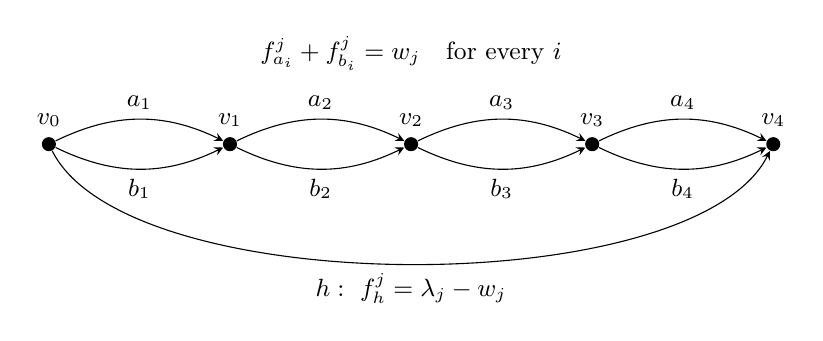
\begin{tikzpicture}[>=stealth,vertex/.style={circle,fill=black,inner sep=1.8pt},
                   every node/.style={font=\small}]
\foreach \i in {0,...,4}{
  \node[vertex,label=above:{$v_\i$}] (v\i) at (2.3*\i,0) {};
}
\foreach \i [evaluate=\i as \prev using int(\i-1)] in {1,...,4}{
  \draw[->] (v\prev) to[bend left=26] node[above] {$a_\i$} (v\i);
  \draw[->] (v\prev) to[bend right=26] node[below] {$b_\i$} (v\i);
}
\draw[->] (v0) .. controls (1,-2.0) and (8.2,-2.0) ..
  node[below] {$h:\ f_h^j=\lambda_j-w_j$} (v4);
\node at (4.6,1.15) {$f_{a_i}^j+f_{b_i}^j=w_j\quad\text{for every }i$};
\end{tikzpicture}
\caption{The flat chain $G_4$. Each serial pair carries the same statewise
branch flow $w_j$; the bypass carries the remainder. All capacities and the
source--sink flow value are one. Independent scalar totals at the four pairs
do not retain the common vector of state flows. The general $G_L$ extends
the same pattern to $L$ pairs.}\label{fig:flat-chain}
\end{figure}

\Cref{fig:flat-chain} illustrates the common profile on $G_4$, which also
supports the coefficient-two example below.

\subsection{A balanced-incidence construction}

\begin{lemma}[Balanced incidence gives a coordinate-section edge]\label{lem:balanced-incidence}
Let $K\in\{0,1\}^{N\times N}$ be invertible, with every row nonempty
and proper. Suppose $\alpha\in\Q_{>0}^N$ and $\beta>0$ satisfy
$K^\top\alpha=\beta\one$. On $G_N$ there is a sparse observation
pattern with $m=N$ such that, for any two distinct rows $r,s$, a
coordinate section has locally the edge
\begin{equation}\label{eq:balanced-edge}
 \alpha_r(U-c)+\alpha_s(V-c)\ge0,
 \qquad c=1/(8N).
\end{equation}
Here $U,V$ are individual observed products, one from each row;
every other original coordinate is fixed. Consequently the hull has a
relative facet with product-coefficient ratio $\alpha_r/\alpha_s$,
invariant under affine-hull equations.
\end{lemma}
\begin{proof}
Put $a=1/(2N)$ and let $S_i=\{j:K_{ij}=1\}$. Fix
$y_j=2a=1/N$ for $j\in[N]$, so the residual state is zero.
Observe $(a_i,j)$ precisely when $j\notin S_i$. Since each $S_i$
is proper, choose one such cell in row $r$ and one in row $s$ as
$U,V$. Fix all other observations to $c=a/4$, and fix
\begin{equation}\label{eq:balanced-aggregate}
 x_h=1/2,\qquad
 x_{a_i}=|S_i|a+(N-|S_i|)c,\qquad
 x_{b_i}=1/2-x_{a_i}.
\end{equation}
All these arc flows are strictly between zero and $1/2$, except for
the stated bypass value. Write $\delta_r=U-c$, $\delta_s=V-c$,
and $\delta_i=0$ in other rows. Since each unobserved $a_i$ entry
is at most its branch profile, every feasible state decomposition obeys
\[
 K(w-a\one)\ge-\delta,\qquad \one^\top w=1/2.
\]
Multiplication by $\alpha^\top$ proves
$\alpha^\top\delta\ge0$, which is \eqref{eq:balanced-edge}.

We prove the converse in an open neighborhood of $(U,V)=(c,c)$.
Put $R=\alpha_r/\alpha_s$, let $\tau$ be zero except for
$\tau_s=R\delta_r+\delta_s$, and define
\begin{equation}\label{eq:balanced-recovery}
 d'=K^{-1}(-\delta+\tau),\qquad w=a\one+d'.
\end{equation}
On the proposed feasible side, $\tau_s\ge0$. Also
$\beta\one^\top d'=\alpha^\top(-\delta+\tau)=0$,
so the profile sums to $1/2$.
For example, with $K_*:=\|K^{-1}\|_\infty$, the neighborhood
\[
 |\delta_r|,|\delta_s|<
 \varepsilon:=\frac{a}{16(1+R)(1+K_*)}
\]
ensures $\|d'\|_\infty<a/16$ and $0\le\tau_s<a/16$.
Indeed $-\delta+\tau$ has only entries $-\delta_r$ and
$R\delta_r$. Every observed value then lies strictly between zero
and $a/2$, whereas each $w_j$ lies between $15a/16$ and $17a/16$.

Initially set $f^j_{a_i}=w_j$ for $j\in S_i$ and set the other
entries to their prescribed observations. The aggregate of row $i$
is $x_{a_i}+\tau_i$, by \eqref{eq:balanced-recovery}.
In row $s$ reduce one entry with $j\in S_s$ by $\tau_s$;
such a state exists and its entry remains nonnegative. All $a_i$
entries are now in $[0,w_j]$ and have the required aggregates.
Set $f^j_{b_i}=w_j-f^j_{a_i}$ and $f^j_h=2a-w_j$.
These are nonnegative, at most $2a$, and satisfy every state balance,
aggregate, and observation. The residual flow is zero. Disaggregation
proves sufficiency, including points on the boundary line. The local
section has two-dimensional interior, so \cref{lem:section-facet}
gives the final claim.
\end{proof}

\begin{example}[Five vertices and nine arcs]\label{ex:small-sp}
Take $N=4$ and
\[
 S_1=\{1,2,3\},\quad S_2=\{1,4\},\quad
 S_3=\{2,4\},\quad S_4=\{3,4\}.
\]
The incidence matrix is invertible: its last three homogeneous row
equations give $d'_1=d'_2=d'_3=-d'_4$, and its first gives
$3d'_4=0$. The balancing weights are $(2,1,1,1)$ with $\beta=3$.
There are seven observations on $G_4$, which has five vertices,
nine arcs, and cycle rank five. With $U=z_{a_1,4}$ and
$V=z_{a_2,2}$, the section edge is $2U+V\ge3/32$.
Here $x_{a_1}=13/32$, $x_{a_i}=5/16$ for $i=2,3,4$,
$x_h=1/2$, and each explicit weight is $1/4$.
More generally, use $N=k+1$, $S_1=[k]$, and
$S_{i+1}=\{i,k+1\}$ for $i\in[k]$, with $k\ge3$.
The same kernel argument proves invertibility and the weights
$(k-1,1,\ldots,1)$ balance every column to $k$. This gives ratio
$M=k-1$, with $M+3$ vertices, $2M+5$ arcs, $M+2$ explicit
states, and $1+M(M+1)$ observations. The next construction attains
exponential ratios with only linearly many observations.
\end{example}

\begin{remark}[Why separate scalar composition fails]\label{rem:scalar-failure}
In \cref{lem:balanced-incidence}, put $U=c-\eta$, $V=c$ for
sufficiently small $\eta>0$. The joint section is infeasible because
$\alpha^\top\delta=-\alpha_r\eta<0$. Nevertheless, each serial
gadget is individually feasible with total branch flow $1/2$ and
the same prescribed state weights. In row $r$, start from the nominal
profile $a\one$ and move $\eta$ of profile mass from a state outside
$S_r$ to a state in $S_r$. Keep the prescribed observed entries,
and fill the entries in $S_r$ to their new profiles. The observed
row total decreases by $\eta$ and the unobserved total increases
by $\eta$, so the aggregate is unchanged. All bounds remain valid
for small $\eta$, including if the donor is the free observed state.
Every other gadget uses the nominal profile. Thus independently
eliminating profiles and passing only their total between gadgets
accepts this infeasible point. The missing information is a single
\emph{common} profile, not a scalar flow balance.
\end{remark}

\subsection{A sparse Fibonacci family}

\begin{theorem}[Exponential ratios on a flat series--parallel chain]\label{thm:fibonacci}
For every $q\ge3$ there is an instance on $G_{2q-1}$ with $m=2q-1$
and $5q-4$ observed products such that every finite original-coordinate
inequality description contains product coefficients in ratio $F_q$,
where $F_1=F_2=1$ and $F_i=F_{i-1}+F_{i-2}$. The graph has $2q$
vertices, $4q-1$ arcs, and cycle rank $2q$. It is planar and has
treewidth two. The original sparse input has encoding length
$O(q\log q)$ and only numerical data in $\{-1,0,1\}$.
\end{theorem}
\begin{proof}
Put $N=2q-1$ and form a square $0/1$ incidence matrix $D$.
Its primary rows are $P_1,\ldots,P_q$ and its auxiliary rows are
$H_0,H_3,\ldots,H_q$. Its columns are
the following subsets of the row set, in the displayed order:
\begin{equation}\label{eq:fibonacci-columns}
 \{H_0,P_1\},\ \{H_0,P_2\};\qquad
 \{H_i,P_i\},\ \{H_i,P_{i-1},P_{i-2}\} (3\le i\le q);
 \qquad \{P_q,P_{q-1}\}.
\end{equation}
There are $2+2(q-2)+1=N$ columns and $4+5(q-2)+2=5q-4$
ones. Each row has two or three ones and each column has two or
three ones, so every row and column is nonempty and proper.
Set $\gamma=F_{q+1}$ and
\[
 \alpha_{P_i}=F_i,\qquad
 \alpha_{H_0}=\gamma-1,\qquad
 \alpha_{H_i}=\gamma-F_i\quad(3\le i\le q).
\]
All weights are positive. The recurrence and the last column show
$D^\top\alpha=\gamma\one$.

To prove invertibility, suppose $D^\top\eta=0$. Subtracting the
first pair of column equations gives $\eta_{P_1}=\eta_{P_2}$;
subtracting each subsequent pair gives
$\eta_{P_i}=\eta_{P_{i-1}}+\eta_{P_{i-2}}$.
Thus $\eta_{P_i}=F_i\eta_{P_1}$. The last column then gives
$F_{q+1}\eta_{P_1}=0$. Every primary and auxiliary entry is zero.

We use the complement $K=\one\one^\top-D$ as the allowed-set
matrix in \cref{lem:balanced-incidence}; consequently its \emph{observed}
cells are precisely the sparse ones of $D$. Put $\sigma=\one^\top\alpha$.
Summing the weights gives $\sigma=(q-1)\gamma+1$, whence
\[
 K^\top\alpha=(\sigma-\gamma)\one,
 \qquad \sigma-\gamma=(q-2)\gamma+1>0.
\]
The complement is invertible. Indeed, if $K^\top\eta=0$, then
$D^\top\eta=(\one^\top\eta)\one$, so
$\eta=(\one^\top\eta)\alpha/\gamma$. Summing this identity and
using $\sigma>\gamma$ forces $\one^\top\eta=0$ and then $\eta=0$.
Its rows are nonempty and proper as required.

Choose $U$ in row $P_q$ and the last column of
\eqref{eq:fibonacci-columns}, and $V$ in row $P_1$ and the first
column. These cells are observed. The exact local section is
\begin{equation}\label{eq:fibonacci-edge}
 F_q U+V\ge(F_q+1)c,\qquad c=1/(8N).
\end{equation}
The facet conclusion follows from \cref{lem:balanced-incidence}.
The graph and observation counts follow from the definition of $G_N$.
Its underlying simple graph is a cycle. Explicit bags
$\{v_0,v_i,v_{i+1}\}$ for $0\le i<N$, in their natural path order,
give a tree decomposition of width two; for $N\ge3$ the cycle
requires that width. Parallel arcs do not affect treewidth or planarity.
All graph, state, and observation lists have $O(q)$ entries, with
indices of $O(\log q)$ bits. The model itself uses only unit data;
even the fixed section coordinates in \eqref{eq:balanced-aggregate}
have $O(\log q)$ bits. Since $F_q$ grows exponentially, the
required integer coefficient magnitudes are superpolynomial in the
input length, while their bit lengths need only grow linearly in $q$.
\end{proof}

The matrix $D$ itself also satisfies \cref{lem:balanced-incidence}
and gives the ratio $F_q$, by choosing any observed cell in each
of rows $P_q,P_1$. That version uses $N^2-(5q-4)$ observations.
Passing to its invertible complement preserves the balancing weights
and makes the observation set sparse.

\begin{corollary}[Simple graphs of maximum degree three]\label{cor:fibonacci-simple}
The same ratio $F_q$ can be realized on a simple acyclic directed
two-terminal series--parallel unit-flow network of maximum undirected
degree three, with $6q-3$ vertices, $8q-4$ arcs, unchanged cycle
rank $2q$, and the same states and observed products.
\end{corollary}
\begin{proof}
In $G_N$, split each of the $N-1$ internal joins into an incoming
vertex and an outgoing vertex connected by a new forward arc.
Subdivide each $b_i$ once. The resulting graph has $3N$ vertices
and $4N$ arcs. The subdivisions remove the parallel pairs; terminals
and split joins have degree three, and subdivision vertices have
degree two. All arcs point forward. The construction remains
two-terminal series--parallel and planar. Such graphs have treewidth
at most two: inductively keep a bag containing the two terminals,
join two such bags for parallel composition, and add the bag
$\{s,v,t\}$ for a series composition through $v$.

Every old flow has a unique extension: each connector carries the
chain flow and each subdivided arc carries the old $b_i$ flow.
Conversely contraction recovers the old flow. The new unit capacities
are redundant because these are nonnegative unit flows on an acyclic
network. The same statements hold separately for every state flow.
All observed $a_i$ arcs remain unchanged. In the coordinate section,
fix each connector to $1/2$ and each new subdivision coordinate to
the corresponding old aggregate. Thus precisely the same free
$(U,V)$ section is obtained, and \cref{lem:section-facet} preserves
its facet-ratio conclusion. Substituting $N=2q-1$ gives the counts.
\end{proof}

The hulls in this section are again $0/1$ polytopes, by the path
argument following \cref{cor:universal-coefficients}. The obstruction
does not conflict with integrality results for aggregate multiflows
on series--parallel digraphs. \citet[Remark~1]{AlmoghrabiSkutellaWarode2026}
explicitly distinguish aggregate arc flows from the full commodity-flow
vector. Here prescribed entries of that state vector carry the
obstruction. The exponential construction lets both block cycle rank
and the number of states grow; it does not disprove a bound at fixed
state count. We next show that a fixed state count does control this
flat topology.

\section{Exact hulls for chains with few observed labels}\label{sec:fixed-chains}

For the same graph $G_L$, arbitrary observations on either gadget arc
and on the bypass admit a small common-profile description. Eliminating
the residual profile coordinate sharpens the general determinant bound
and gives a unit-coefficient original hull when $m\le3$.

\subsection{The complete shared-profile system}

First check $x\in\Flow$, $y\in\Delta_m$, and $z\ge0$ on the
observed coordinates. These conditions are part of every description
below. Put $t=1-x_h$, and index all $d=m+1$ states by $\states$.
For each gadget $i$, partition the states into $A_i,B_i,T_i,U_i$:
only $a_i$ is observed, only $b_i$ is observed, both are observed,
or neither is observed, respectively. In particular $0\in U_i$.
Write $u_{ij}=z_{a_i,j}$ and $v_{ij}=z_{b_i,j}$ wherever present,
and define
\begin{equation}\label{eq:chain-R}
 R_i=x_{a_i}-\sum_{j\in A_i\cup T_i}u_{ij}
                  +\sum_{j\in B_i}v_{ij}.
\end{equation}
The use of $T_i$ for a state class is unrelated to the table polytope
$\mathcal T$ in \cref{sec:universality}.

\begin{proposition}[Exact profile formulation]\label{prop:chain-profile}
Subject to the preceding original-domain checks, $(x,y,z)\in\Hull$
if and only if there is $w\in\R^{m+1}$ satisfying
\begin{align}
 0\le w_j\le\lambda_j\quad(j\in\states),\qquad
 &\sum_{j\in\states}w_j=t,\label{eq:chain-profile-bounds}\\
 w_j&=\lambda_j-z_{h,j}&&((h,j)\in\Obs),\label{eq:chain-bypass}\\
 w_j&\ge u_{ij}&&(j\in A_i),\nonumber\\
 w_j&\ge v_{ij}&&(j\in B_i),\nonumber\\
 w_j&=u_{ij}+v_{ij}&&(j\in T_i),\label{eq:chain-cells}\\
 \sum_{j\in B_i}w_j\le R_i&\le
       \sum_{j\in B_i\cup U_i}w_j&&(i\in[L]).\label{eq:chain-endpoints}
\end{align}
\end{proposition}
\begin{proof}
Every state disaggregation supplies its profile through
\eqref{eq:chain-profile}. Its observed entries give
\eqref{eq:chain-bypass}--\eqref{eq:chain-cells}. In gadget $i$,
the $a_i$ entries are $u_{ij}$ in $A_i\cup T_i$, are $w_j-v_{ij}$
in $B_i$, and are free in $[0,w_j]$ in $U_i$. Thus their possible
aggregate is exactly the interval
\[
 \left[\sum_{A_i\cup T_i}u_{ij}+\sum_{B_i}(w_j-v_{ij}),\quad
 \sum_{A_i\cup T_i}u_{ij}+\sum_{B_i}(w_j-v_{ij})+
 \sum_{U_i}w_j\right].
\]
Membership of $x_{a_i}$ in this interval is
\eqref{eq:chain-endpoints}.
Conversely these inequalities allow the free $U_i$ entries to be
chosen with the required sum, independently for each gadget. All
entries lie in $[0,w_j]$: for a doubly observed state this follows
from $w_j=u_{ij}+v_{ij}$ and the original nonnegativity check.
Set every $b_i$ entry to $w_j-f^j_{a_i}$ and the bypass entry to
$\lambda_j-w_j$. State capacities and balances hold, and
$x_{a_i}+x_{b_i}=t$ supplies each $b_i$ aggregate. The bypass
aggregate is $\sum_j\lambda_j-t=x_h$. This is a complete
disaggregation. If a weight is zero, its profile and all its entries
are zero, so no positive-weight assumption has been used.
\end{proof}

Eliminate the unobserved residual coordinate by
$w_0=t-\sum_{j=1}^mw_j$, and write $\widehat w=(w_1,\ldots,w_m)$.
The residual bounds become
\begin{equation}\label{eq:chain-residual-reduced}
 \one^\top\widehat w\le t,\qquad
 -\one^\top\widehat w\le\lambda_0-t.
\end{equation}
Since $0\in U_i$, the endpoint rows become
\begin{equation}\label{eq:chain-endpoints-reduced}
 \one_{B_i}^\top\widehat w\le R_i,\qquad
 \one_{A_i\cup T_i}^\top\widehat w\le t-R_i.
\end{equation}
All remaining rows have singleton normals $\pm e_j$.
Thus each nonzero normal belongs to the fixed universe
\begin{equation}\label{eq:chain-normal-universe}
 \mathcal N_m=\{\one_S:\varnothing\ne S\subseteq[m]\}
                 \cup\{-e_j:j\in[m]\}\cup\{-\one\}.
\end{equation}
Repeated normals represent different affine right-hand sides; keep
the minimum of these right-hand sides at a query point. A zero
normal gives a scalar inequality and must be checked separately.
Every original flow or product has coefficient in $\{-1,0,1\}$
in every individual right-hand side, including $t-R_i$.

\subsection{Finite circuits and constructive recovery}

Let $\Delta^{01}_m$ be the maximum absolute determinant of a square
$0/1$ matrix of order at most $m$, including the empty determinant
one. In particular $\Delta^{01}_1=\Delta^{01}_2=1$, $\Delta^{01}_3=2$, and
$\Delta^{01}_m\le\max(1,m^{m/2})$ by Hadamard's inequality.

\begin{theorem}[Fixed-state chain hull and recovery]\label{thm:fixed-chain}
For $m\ge1$, the sparse hull on $G_L$ has a finite
original-coordinate description with integer flow and product
coefficients of magnitude at most $(m+1)\Delta^{01}_m$.
After $2^{O(m^2)}$ preprocessing depending only on $m$, exact
separation and state-flow recovery each require
\[
 O(mL+|\Obs|+m)+2^{O(m^2)}
\]
rational arithmetic operations. Recovery calls no online linear
program. Rational encoding lengths remain polynomial in the input
length. For $m=0$, the hull is simply the original flow polytope.
\end{theorem}
\begin{proof}
Form the reduced profile inequalities
$a^\top\widehat w\le\gamma_a$ for the distinct present nonzero
normals, where $\gamma_a$ is the minimum of all right-hand sides
with normal $a$. There are at most $2^m+m$ such normals.
The system is feasible exactly when all its nonnegative cancellation
certificates have nonnegative right-hand side, by Farkas' lemma.
The cone of such certificates is
\[
 \{\mu\ge0:\ \sum_a\mu_a a=0\}.
\]
It is pointed. Each extreme ray has minimally dependent support,
of size at most $m+1$; otherwise a linear dependence within its
support permits a small perturbation in both directions and contradicts
extremality. Conversely every minimal positive dependence gives such
an extreme ray. We call these supports, with their primitive positive
integer weights, \emph{positive circuits}.

For a support of size $s$, select $s-1$ independent columns in
its row matrix. The signed $(s-1)$-row minors give a nonzero kernel
vector and hence its circuit weights after a common sign change and
division by the greatest common divisor. Each row is a $0/1$ vector
or its negative. Changing whole-row signs bounds every such minor
by $\Delta^{01}_m$. Therefore every primitive weight is at most
$\Delta^{01}_m$. The extreme rays generate the certificate cone, so
the finitely many tests
\begin{equation}\label{eq:chain-circuit-tests}
 \sum_{a\in C}\mu_a\gamma_a\ge0
 \quad\text{for every positive circuit $C$ of present normals}
\end{equation}
are necessary and sufficient, together with the scalar zero-row
checks. Each circuit is one in the full fixed universe
\eqref{eq:chain-normal-universe}.

Expanding \eqref{eq:chain-circuit-tests} over all choices of an
original row for each participating normal gives a finite affine
description. Positivity of the weights makes this expansion exact:
the weighted sum of minima is the minimum over independent choices.
Each affine inequality sums at most $m+1$ rows, with weights at
most $\Delta^{01}_m$, and hence has the claimed original-coordinate
coefficient bound. At an infeasible query it suffices to output the
rows attaining the minima in one violated circuit. This produces
a globally valid affine inequality, even though other rows may
attain the minima at other points. The original-domain prechecks
have unit coefficients as well.

Enumerate all supports of size at most $m+1$ in the fixed universe,
and use exact elimination to keep their positive circuits. There
are $2^{O(m^2)}$ candidates. Constructing and grouping the profile
rows takes $O(mL+|\Obs|+m)$ arithmetic operations; the circuit
tests then have parameter-only cost $2^{O(m^2)}$.
For this count, preindex subset normals by bit masks and cache the
singleton indices. A scan of each gadget builds its two subset masks
and right-hand sides, while each local cell row uses a cached index;
one need not copy an $m$-entry normal for every local row. The masks
have $O(m)$ bits, which is included in the polynomial bit-length
qualification below.

For recovery, also precompute inverses of all nonsingular matrices
formed by $m$ distinct normals of $\mathcal N_m$. At a feasible
query enumerate those whose rows are present and solve their
equalities against the corresponding grouped right-hand sides.
Test each candidate against all the grouped inequalities, and keep
the first feasible candidate. This succeeds: the profile polyhedron
is nonempty and bounded by $0\le w_j\le\lambda_j$, so has a
vertex; at a vertex the active normals span $\R^m$, even if the
polyhedron is lower dimensional. If they failed to span, a sufficiently
small displacement in a nonzero orthogonal direction and its negative
would remain feasible, contradicting that it is a vertex. Thus the
enumeration includes that vertex. Its number of candidates and all
candidate tests are bounded by $2^{O(m^2)}$.

Set $w_0=t-\sum_{j=1}^mw_j$. In each gadget, the remaining
$U_i$ entries must sum to
$R_i-\sum_{B_i}w_j\in[0,\sum_{U_i}w_j]$. Fill these entries
in any fixed order, repeatedly taking the smaller of the remaining
sum and $w_j$. This takes $O((m+1)L)$ arithmetic operations and
gives the disaggregation in \cref{prop:chain-profile}. Divide
positive-weight states by their weights to obtain at most $m+1$
graph points, omitting zero states. Writing all state-arc entries
has this same $O((m+1)L)$ output scale.

All bases have integer entries of magnitude at most one. Their
inverses have cofactors bounded by $\Delta^{01}_m$ and nonzero integer
determinants bounded by $\Delta^{01}_m$. Grouping selects input-derived
affine right-hand sides; circuit tests and inverse-basis recovery
therefore use numbers with polynomial encoding length. Greedy filling
uses only additions, comparisons, and minima of these rational values.
Normalization by positive rational weights preserves polynomial
encoding length. The arithmetic parameter dependence is exponential,
but no unbounded-precision unit-cost assumption is needed for the
bit-length assertion.
\end{proof}

\begin{remark}[The unreduced signed-subset library]\label{rem:unreduced-chain}
Keeping all $d=m+1$ profile coordinates yields normals
$\{\pm\one_S:\varnothing\ne S\subseteq\states\}$.
The same proof gives the bound $(d+1)\Delta^{01}_d$ and
$2^{O(d^2)}$ parameter work. Its positive-circuit counts for
$d=1,2,3$ are respectively $1,5,41$, with largest primitive
weights $1,1,2$. These are counts of the full signed-subset universe,
not of the rows that necessarily occur in a particular instance.
Eliminating the residual coordinate gives the smaller universe
\eqref{eq:chain-normal-universe}: for $m=1,2,3$ it has
$2,6,11$ normals and $1,5,16$ positive circuits, respectively,
again with largest weights $1,1,2$. The stated finite enumeration
reproduces these counts exactly; they are not assumptions in the
proof. In particular the 41-circuit library is unnecessary for a
chain with two explicit states.
\end{remark}

\subsection{Two explicit states: five tests and unit coefficients}

For $m=2$, the reduced normal universe is just
$\{\pm e_1,\pm e_2,\pm(e_1+e_2)\}$. After grouping, the
profile region takes the form
\begin{equation}\label{eq:chain-hexagon}
 \ell_1\le w_1\le u_1,\qquad
 \ell_2\le w_2\le u_2,\qquad
 \ell_s\le w_1+w_2\le u_s.
\end{equation}
All six endpoint groups are present because of the explicit and
residual weight bounds. This is the same three-direction geometry
used in the theta oracle, but here the individual profile region
itself describes all serial gadgets together.

\begin{theorem}[Unit coefficients and a five-test chain oracle]\label{thm:two-state-chain}
On $G_L$ with at most two explicit simplex variables and arbitrary
observations, the sparse hull has a finite exact description with
all flow and product coefficients in $\{-1,0,1\}$.
With two explicit variables, after the original-domain and zero-row
checks, membership is equivalent to the five conditions
\begin{equation}\label{eq:chain-five-tests}
 \ell_1\le u_1,\quad \ell_2\le u_2,\quad
 \ell_s\le u_s,\quad
 \ell_1+\ell_2\le u_s,\quad
 \ell_s\le u_1+u_2.
\end{equation}
Exact separation and constructive decomposition take
$O(L+|\Obs|+1)$ rational arithmetic operations, with no circuit
enumeration and no online linear program.
\end{theorem}
\begin{proof}
The possible sum of two interval variables is
$[\ell_1+\ell_2,u_1+u_2]$. Thus \eqref{eq:chain-five-tests}
are exactly the conditions that both intervals are nonempty and
this sum interval meets $[\ell_s,u_s]$. On a feasible query set
\[
 s_* =\max(\ell_s,\ell_1+\ell_2),\qquad
 w_1=\max(\ell_1,s_*-u_2),\qquad w_2=s_*-w_1.
\]
The tests ensure $s_*\le\min(u_s,u_1+u_2)$, and these choices
satisfy every bound in \eqref{eq:chain-hexagon}. Complete the
flows by the greedy construction in \cref{thm:fixed-chain}.

We must check original coefficients, since unit circuit weights alone
would not exclude repeated occurrences of the same product. The five
positive circuits are the three opposite pairs and
\begin{equation}\label{eq:chain-five-circuits}
 \{e_1,e_2,-\one\},\qquad
 \{-e_1,-e_2,\one\},
\end{equation}
all with weights one. The following occurrence analysis applies to
any affine row selected in each normal group. No circuit contains
both $-e_j$ and $+e_{3-j}$, or both $+e_j$ and $+\one$.

For an $a_i$ product in an only-$a_i$ state $j$, its negative
occurrences are in the local row $-e_j$ and the endpoint row
$+\one_{B_i}$; since $j\notin B_i$, the latter is either zero
or $+e_{3-j}$. Its only positive occurrence is in the other endpoint
row $+\one_{A_i\cup T_i}$. Thus a circuit cannot select two
negative occurrences. If state $j$ is doubly observed, the positive
local row $+e_j$ is also available. The other positive normal
contains $j$, so is either the same normal $+e_j$ or $+\one$;
one row is selected per normal, and these two distinct normals do
not occur together in a circuit. The negative occurrences remain
as above. Hence every $a_i$ product has coefficient of magnitude
at most one.

For a $b_i$ product in an only-$b_i$ state $j$, the negative
occurrences are $-e_j$ and $+\one_{A_i\cup T_i}$, whose latter
normal excludes $j$; the positive occurrence is the $B_i$ endpoint.
The same argument applies. A doubly observed $b_i$ product occurs
only in the two opposite local singleton rows, with opposite signs,
because $R_i$ uses the observed $a_i$ entry in that state.
A bypass product likewise occurs only in two opposite singleton rows.
Each zero-row inequality separately has unit coefficients.

The coordinate $x_{a_i}$ occurs only in its two endpoint rows,
once with each sign, and $x_{b_i}$ occurs only in the original
flow precheck. The shared coordinate $x_h$ needs an additional
check. In a positive singleton row its coefficient is zero or
$-1$, in a negative singleton row it is zero, in the positive
full row it is zero or $-1$, and in the negative full row it is
always $+1$. These statements follow by inspecting
\eqref{eq:chain-residual-reduced} and
\eqref{eq:chain-endpoints-reduced}; for example a full $B_i$
endpoint has zero $x_h$ coefficient, whereas a full $A_i\cup T_i$
endpoint has coefficient $-1$.
For the first circuit in \eqref{eq:chain-five-circuits}, two
negative contributions from its positive singleton rows are offset by the compulsory
$+1$ from the negative full row. All opposite pairs and the
second circuit also have coefficient magnitude at most one.
Consequently every affine branch of the five tests is a unit
flow/product inequality, proving the claimed finite description.

For $m=1$ the reduced system is an interval. Alternatively, embed
it as the coordinate section $y_2=0$ of the two-state instance
with no observations in label 2. Disaggregation forces state 2
to zero, so restriction of the established unit description is
exact and preserves its flow/product coefficients. The case $m=0$
is the original flow description. Grouping rows, checking the five
tests, and filling the state flows have the asserted linear cost.
\end{proof}

\subsection{Three explicit states and a sharp state-count threshold}

The coefficient conclusion extends one state further. In this case
some direct circuit sums have bypass-flow coefficient two, but a
single original flow equation removes it. This is a valid change of
an ambient inequality representative, in contrast to changing either
free coefficient in the coordinate sections of
\cref{lem:section-facet}.

\begin{theorem}[Sharp unit-coefficient threshold for flat chains]\label{thm:three-state-chain}
For arbitrary observations on $G_L$, three explicit simplex variables
still admit a finite exact original-coordinate description with unit
flow and product coefficients. At most sixteen fixed positive-circuit tests,
with the original-domain and zero-row checks, give exact separation
and constructive recovery in $O(L+|\Obs|+1)$ rational arithmetic
operations. Four explicit variables already allow a hull with no
such unit-coefficient description.
\end{theorem}
\begin{proof}
For $m=3$, the positive circuits of \eqref{eq:chain-normal-universe}
have the following four forms. Each listed normal has weight one
unless specified otherwise:
\begin{align}
 &\{\one_S\}\cup\{-e_j:j\in S\}
       &&(\varnothing\ne S\subseteq[3]);\label{eq:chain3-circuits-a}\\
 &\{-\one\}\cup\{\one_S:S\in\pi\}
       &&(\pi\text{ a partition of }[3]);\label{eq:chain3-circuits-b}\\
 &\{-\one,-e_i,e_i+e_j,e_i+e_k\}
       &&(\{i,j,k\}=[3]);\label{eq:chain3-circuits-c}\\
 &\{-\one,e_1+e_2,e_1+e_3,e_2+e_3\},
       &&\text{weight two on }-\one.\label{eq:chain3-circuits-d}
\end{align}
Their numbers are $7,5,3,1$. Here is a direct completeness check.
Without $-\one$, a positive dependence decomposes into the
dependencies of each positive subset on its negative singleton
coordinates, so minimality leaves exactly
\eqref{eq:chain3-circuits-a}. With $-\one$, presence of $+\one$
forces the opposite pair. Otherwise there are at most three other
normals, by the circuit support bound. Two negative singleton
normals would leave at most one positive proper subset, which
cannot cover all three coordinates and also supply an excess in
either negative singleton coordinate. With one negative singleton
$-e_i$, two positive subsets are necessary. The opposite singleton
$+e_i$ is excluded by minimality. The coordinate equations then
force the positive subsets to be $\{i,j\}$ and $\{i,k\}$,
giving \eqref{eq:chain3-circuits-c}. With no negative singleton,
the positive subsets form a minimal uniformly weighted cover.
If a singleton is present, overlapping pairs would force one of
their other coordinates to exceed the common cover value, so the
sets form a partition. With only pairs, all three pairs are needed,
and their equal weights give \eqref{eq:chain3-circuits-d}.
This also verifies positivity and minimality of the displayed list.

All positive-normal weights are one. No circuit contains both
$-e_j$ and a positive subset normal excluding $j$, or both
$+e_j$ and a different positive subset normal containing $j$.
These facts follow immediately from the four forms. The occurrence
argument in \cref{thm:two-state-chain} therefore proves that every
product coefficient has magnitude at most one for every choice of
affine branches. The only doubled circuit weight belongs to
$-\one$, whose right-hand side $\lambda_0-t$ has no product
coordinate. Each $x_{a_i}$ has at most its two opposite-signed
endpoint occurrences, each with weight one, and no $x_{b_i}$
occurs in a profile right-hand side.

It remains to handle $x_h$. Negative singleton rows have coefficient
zero; the negative full row has coefficient $+1$. A positive
subset row has coefficient zero or $-1$. Thus circuits
\eqref{eq:chain3-circuits-a} and \eqref{eq:chain3-circuits-c}
have unit $x_h$ coefficients. In
\eqref{eq:chain3-circuits-b}, the only exception is coefficient
$-2$: the partition must consist of three singletons and all three
chosen right-hand sides must be upper endpoints $t-R_i$.
They belong to distinct gadgets, since each gadget supplies only
one upper endpoint. Choose one of them. Its $x_{a_i}$ coefficient
is $-1$, with no other contribution from that gadget. In the
circuit inequality written as an affine expression at least zero,
add the identically zero flow expression
\[
 x_{a_i}+x_{b_i}+x_h-1.
\]
The coefficients of $x_h,x_{a_i},x_{b_i}$ become $-1,0,1$.

In \eqref{eq:chain3-circuits-d}, the only exception is coefficient
$+2$, occurring when all three positive pair rows have zero
$x_h$ coefficient. A positive pair row can only come from a
gadget endpoint, so these are three lower endpoints $R_i$ from
distinct gadgets. Choose one and subtract its flow expression
$x_{a_i}+x_{b_i}+x_h-1$. The three affected coefficients become
$1,0,-1$. No other coefficient changes. These replacements preserve
validity on the original flow domain and leave the violation at any
query that passes the flow precheck unchanged. Hence every branch
of the exact circuit description has a unit-coefficient representative.

The circuit and inverse-basis libraries now have fixed size.
\Cref{thm:fixed-chain} supplies linear-cost separation and recovery,
including zero weights and lower-dimensional profile regions.
Finally \cref{ex:small-sp} has four explicit states and a local
section normal $(2,1)$. By \cref{lem:section-facet}, this ratio
cannot be removed by any affine-hull equation, so no unit-coefficient
description exists. Additional unused explicit variables can be
fixed to zero if a counterexample with more than four is desired.
\end{proof}

\begin{example}[Both bypass-coefficient repairs are needed]\label{ex:chain3-repairs}
Take $L=3$, $x_h=1/2$, and first let $y_1=y_2=y_3=1/3$,
$x_{a_i}=2/5$, $x_{b_i}=1/10$. Observe only $(a_i,i)$,
with all three products zero. The singleton-partition certificate is
\[
 \sum_{i=1}^3(t-R_i)+(\lambda_0-t)
   =2t-\sum_{i=1}^3x_{a_i}+\sum_{i=1}^3z_{a_i,i}+\lambda_0
   =-1/5.
\]
It has $x_h$ coefficient $-2$; adding any selected gadget balance
gives a unit-coefficient violated inequality.
For the other repair, take $y_1=y_2=y_3=1/4$,
$x_{a_i}=1/20$, $x_{b_i}=9/20$. Observe only $b_i$ products,
on state pairs $\{1,2\},\{1,3\},\{2,3\}$ in gadgets 1, 2, 3,
respectively, each with value $1/20$. Now $R_i=3/20$ and the
pair-triangle certificate is
\[
 R_1+R_2+R_3+2(\lambda_0-t)=-1/20.
\]
Its $x_h$ coefficient is $+2$; subtracting a selected gadget
balance gives the unit form. Both query points satisfy all original
flow, simplex, and separate McCormick inequalities. The exact
joint cuts detect the missing common profile.
\end{example}

\begin{corollary}[Only observed labels count]\label{cor:chain-observed-labels}
Let $J=\{j:(e,j)\in\Obs\text{ for some }e\}$ and $a=|J|$.
All fixed-state chain conclusions apply with $a$ in place of $m$.
In particular, at most three observed labels guarantee unit flow/product
coefficients, regardless of the number of unobserved simplex labels;
at most two observed labels permit the five-test oracle.
General separation and compact recovery take
$O((a+1)L+|\Obs|+m)+2^{O(a^2)}$ rational arithmetic operations.
\end{corollary}
\begin{proof}
Apply the exact state merger in \cref{thm:block-state-reduction},
retaining the labels in $J$ and merging all others with the residual
state. The merged weight is $1-\sum_{j\in J}y_j$.
Keep the original simplex constraints on all $m$ coordinates and
apply the preceding theorems to this reduced state list. Substituting
the merged weight changes no flow or product coefficient. The
proportional refinement \eqref{eq:proportional-refinement} recovers
each unused label from the same normalized merged flow. It can be
stored as one flow and its constituent weights, so the stated
compact-recovery cost includes only $O(m)$ additional bookkeeping.
Writing every entry of all global state flows instead can require
$\Theta((m+1)|E|)$ output operations. If $a=0$, the hull is simply
$\Flow\times\Delta_m$ and no profile elimination is needed.
\end{proof}

These theorems are specific to a chain of parallel pairs with one bypass.
A general nested series--parallel construction can require several
interacting profiles. Neither the five-test result nor the
fixed-state determinant bound above asserts a description for that
larger class. Conversely, \cref{thm:fibonacci} shows why a coefficient
bound independent of the state count is impossible even on this
flat family.

\section{Implementation, verification, and computational comparisons}\label{sec:computation}
% Generated by verification/stage06-tables.py; data SHA256 373ce70b3839c12a206b193e9952d856f585da400f902bda773a725a609f73ac
\newcommand{\BenchPython}{3.12.14}
\newcommand{\BenchNumpy}{2.5.2}
\newcommand{\BenchScipy}{1.18.1}
\newcommand{\BenchHullObjective}{-6.981917}
\newcommand{\BenchMcObjective}{-7.287862}
\newcommand{\BenchBudgetObjective}{-6.538573}
\newcommand{\BenchCutCount}{42}
\newcommand{\BenchOldCold}{31.05}
\newcommand{\BenchNewThreeCold}{10.78}
\newcommand{\BenchNewThreeBases}{9.15}


The implementations serve two distinct purposes: constructing small numerical
LPs and producing exact rational hull certificates. The experiments compare
both with strengthened versions of classical disaggregation. They show large
model-size savings, but also cases where a simpler LP is faster and cases where
global state merging explains most of an apparent compression advantage.

\subsection{Implemented scope and certificate semantics}

\begin{table}[tb]\centering\small
\caption{Implemented scope. Exact assembly of an LP does not make its
floating-point optimizer an exact certificate.}\label{tab:implemented-scope}
\begin{tabular}{>{\raggedright\arraybackslash}p{.19\linewidth}>{\raggedright\arraybackslash}p{.36\linewidth}>{\raggedright\arraybackslash}p{.36\linewidth}}\toprule
Component & Supported input & Returned evidence\\\midrule
Parallel-path separator & Arbitrarily oriented multigraphs whose cyclic
blocks are parallel paths; loops and bridges included & Exact original-coordinate
cut or compact rational decomposition\\[3pt]
Flat-chain separator & Canonical unit-data $G_L$, arbitrary observations;
parameter is the number of observed labels & Exact cut or compact decomposition;
unit flow/product coefficients through three observed labels\\[3pt]
General compressed EF & Arbitrary bounded equality-flow graphs; initial
or observed-coordinate-eliminated formulation & Exact rational model;
numerical LP solution; optionally an exactly checked Farkas cut\\[3pt]
Bounded-rank libraries & Supplied small signed-normal systems and structural
verification instances & Verification prototype for support and recovery;
not a complete production general-graph oracle\\\bottomrule
\end{tabular}
\end{table}

\Cref{tab:implemented-scope} distinguishes the three usable interfaces
from the bounded-rank verification code. The specialized separators use
Python's standard library and rational arithmetic throughout. They check
original flow and simplex constraints, retain the original affine expressions
of active bounds, and return a cut with strictly positive exact violation
or a decomposition whose positive-weight normalized flows belong to $\Flow$.
The graph separator rejects unsupported blocks explicitly. The flat oracle
merges unobserved labels, eliminates the residual profile, and uses the
five-test formula when at most two labels are observed. At three labels it
uses the 16 circuits and both flow-balance repairs of
\cref{thm:three-state-chain} for separation. Recovery uses finite inverse
bases at three or more observed labels.
Its stored default is shared across unused global labels. Compatibility
accessors can materialize the former dense state arrays, with the corresponding
output cost. Tuple normal construction and hashing retain a dimension factor
relative to the preindexed-mask operation count in \cref{thm:fixed-chain};
apart from the constructor's $O(|\Obs|\log|\Obs|)$ observation sorting,
the implemented cost is linear in $L$ at fixed observed-label count.

The general formulation stores exact rational coefficients, including the
observed-coordinate substitutions, but calls a numerical LP solver.
Its phase-I certificate routine rationalizes dual weights and, if necessary,
repairs their supported kernel equations by exact elimination. A returned
cut is accepted only after checking nonnegative weights, exact cancellation
of every auxiliary coordinate, and strictly positive rational violation.
The API distinguishes \texttt{certified\_outside},
\texttt{numerically\_feasible}, \texttt{uncertified\_outside}, and
\texttt{solver\_failure}. The second status is not exact membership,
and failure of exact multiplier recovery is not an infeasibility certificate.
This is an implementation of classical Farkas projection, not a new generic
separation theorem.

Code indices are zero based, with explicit states $0,\ldots,m-1$ and
residual state $m$; this is only an indexing change from the manuscript.
The LP baseline generator uses outgoing-minus-incoming balances, and its
adapter negates them before calling either production model. Float inputs
to exact interfaces mean their decimal text. The optimization experiment
uses a small-denominator reconstruction adapter, requires error below
$10^{-7}$ and exact aggregate balances, and then checks the returned
decomposition exactly. This adapter is suitable for the stated synthetic
instances; it is not a general certified rational LP optimizer.

The verification suite compares against independently assembled full-state
LPs and, for small graphs, directly enumerated path--simplex vertices.
The updated flat tests include arbitrary observations and zero weights,
both three-label repairs with exact global cut checks, the four-label
ratio-two obstruction, and sparse observed labels among many original
simplex coordinates. They also test an interior-residual point with zero
explicit profile and positive residual branch flow: this rules out
incorrectly reusing a basis construction that forces the explicit profile
sum to the full branch flow. Separate tests check every new rank-three
inverse basis. The unchanged independent flat audit verifies 192 exact
decompositions and 708 exact violated cuts, with 233 numerical path-hull
comparisons. The general compressed audit passes 600 objective comparisons,
758 membership comparisons, and 476 exactly checked Farkas cuts, each also
tested by numerical full-hull support optimization. Its structural integration
checks recover the coefficient ratios two, five, and twenty-one. These finite
checks support the code; the preceding proofs establish the general claims.

\subsection{Baselines that retain the elementary reductions}

For optimization with fixed weights, the full disaggregation uses only
positive-weight state flows, block balances $Af^j=\lambda_j b$, and native
variable bounds $0\le f^j\le\lambda_j u$. It eliminates $x,z$ by substitution
and adds the constant $c_y^\top\bar y$ to the objective value. In additional
original-coordinate rows, the fixed $y$ contribution moves to the right-hand
side. This is one joint LP and remains valid with the aggregate budget below.
The global-merger baseline first groups labels observed nowhere into one
default, then applies the same construction to its positive-weight states.
With free weights, both interfaces retain every original $y$ variable and its
objective and constraint contributions. Both use sparse block and Kronecker
assembly. They use no graph blocks, cycle coordinates, or observation
rank elimination. Initial compression and observed elimination use the two
variants of the general implementation, including their preprocessing costs.

For point membership, $x,y,z$ are data and only state flows are LP variables.
The historical full baseline already had this property. The strengthened
baseline removes exactly zero-weight states, checks their observations, and
assembles state balances and aggregate equations as sparse block matrices.
It accepts solver statuses zero and two as numerical feasibility and
infeasibility; other statuses are failures, not successful rejections.

An additional elementary baseline applies when precisely two states have
positive weights $\lambda,\mu$, with $\lambda+\mu=1$. After checking
the original aggregate flow, write the state flows as $f$ and $x-f$.
The complete remaining feasibility system is
\begin{equation}\label{eq:two-state-membership-lp}
 Af=\lambda b,\qquad
 \max\{0,x-\mu u\}\le f\le\min\{\lambda u,x\}.
\end{equation}
An observation in the first state fixes $f_e=z_{ej}$; an observation
in the second fixes $f_e=x_e-z_{ej}$. Intersect these fixed values
with both bounds and with each other. The second state's balance follows
from $Ax=b$, so this one-flow network LP is exact as a formulation.
One positive state requires only a direct check. In the numerical implementation
the aggregate balance precheck uses tolerance $10^{-9}$; its LP answer is
still numerical evidence. Exact input arithmetic identifies zero states and
checks the intersected bounds.

Fixed-weight linear optimization without additional coupling is also simpler
than a joint LP suggests. If $c^j_e$ is the product-objective coefficient
for $(e,j)$, or zero when absent, and $c^0=0$, then disaggregation gives
\begin{equation}\label{eq:independent-network-objectives}
 \min_{(x,\bar y,z)\in\Hull}
       (c_x^\top x+c_y^\top\bar y+c_z^\top z)
 =c_y^\top\bar y+
   \sum_{j\in\states}\lambda_j
       \min_{v\in\Flow}(c_x+c^j)^\top v.
\end{equation}
This follows by independently minimizing each positive-weight state flow;
zero-weight terms vanish. Unobserved labels have identical costs and share
one solve. We include this sequential network-LP baseline. With free weights
and no side constraints, a simplex vertex suffices, so such stand-alone
objectives should not be presented as intrinsically difficult coupled problems.

\subsection{Instances and measurement protocol}

All reported data are synthetic. The code uses SciPy
\citep{Virtanen2020} and its bundled HiGHS LP solver
\citep{HuangfuHall2018}, with default \texttt{highs} options.
The recorded versions are Python~\BenchPython, NumPy~\BenchNumpy,
and SciPy~\BenchScipy, on x86-64 Linux under WSL2 with 36 visible
logical CPUs. The bundled HiGHS version is 1.12.0. No affinity, host
isolation, persistent model, or solver warm-start advantage is claimed.
Each case has one recorded warmup followed by five runs with method order
rotated. Each run rebuilds its model. Build and solver times are recorded
separately, together with total times and all minimum/median/maximum values.
Component medians need not add to the total median. Independent certificate
audits occur outside the timed components and have their own recorded cost.
Membership-only and decomposition-inclusive exact queries are separate
workloads, not timings inferred by subtraction.

The principal sparse optimization instance has four articulation-linked
blocks, each containing five internally disjoint paths of length two,
with a bridge between successive blocks. It has 43 arcs and 128 explicit
labels. Capacities are integers from two to eight, orientations vary, and
balances are induced by the half-capacity reference flow. Each block observes
three labels on three arcs each. The graph and label-generation seeds are
fixed in the accompanying generator; the primary seed is 33, and objective
seed 1033 gives independent normal costs with standard deviation $0.15$
on $x$, zero on $y$, and standard deviation one on observed $z$.
Weights are fixed to $9/(10m)$.

The membership family uses four six-path blocks of length two, seed 41,
51 arcs, 36 observations, and $m=16,128,1024$. Each explicit state has
weight $1/(2m)$, leaving residual weight $1/2$. In block $B$, state
$j$ perturbs path $(j+B)\bmod6$ and the next path by opposite amounts
$(j\bmod3-1)/4$, with path orientation signs applied. The aggregate
and observations are formed from this exact mixture around the half-capacity
reference. These are feasible membership queries, not random rejection tests.

Two controls separate the mechanisms. First, an all-labels-observed instance
has 16 three-path blocks, four disjoint labels per block, and one observation
on the first arc of each path for each local label. All 64 labels occur
somewhere, so global merging cannot help. It has 111 arcs and 192 observations;
graph seed 73 and objective seed 1073 are fixed, with nonzero $y$ costs and
weights $9/640$. Second, on the original 43-arc instance, choose the
nonnegative resource indicator $d_e=1$ where an unconstrained optimum has
$x_e$ above the reference value, and zero elsewhere. Put
\[
 d^\top x\le B,\qquad
 B=\tfrac12(d^\top x^{\rm opt}+d^\top x^{\rm ref}).
\]
The exact reconstructed unconstrained point violates this row, while the
reference graph point satisfies it. Every formulation receives the same
aggregate row. This compares equivalent relaxations $\Hull\cap\{d^\top x\le B\}$;
it does not assert that convexification commutes with adding a budget.
The independent-state baseline \eqref{eq:independent-network-objectives}
is inapplicable to this coupled control.

Finally the flat family uses $G_L$ for $L=8,32,128,512$, observing
$(a_i,1)$ and $(a_i,2)$ alternately. Boundary weights are $(1/2,1/2)$;
interior weights are $(1/3,1/3)$, so the latter has three positive
states. Feasible queries have $x_{a_i}=x_{b_i}=1/4$, $x_h=1/2$.
Writing $g=i-1$, the boundary observed value is
$1/8+(-1)^g(g\bmod3-1)/16$; the interior value is
$1/12+(g\bmod3-1)/48$. Branch profiles $1/4,1/4$ in the boundary
case and $1/6,1/6,1/6$ in the interior case give feasible completions:
in the latter, split the remaining $a_i$ aggregate equally between
the other two states. Infeasible queries use
$x_{a_i}=3/10$, $x_{b_i}=1/5$, $x_h=1/2$, and every observed
product $3/10$. All separate McCormick inequalities hold, but the
two observed profiles would sum to at least $3/5>1/2$.

\subsection{Size savings and runtime tradeoffs}

% Generated by verification/stage06-tables.py; data SHA256 373ce70b3839c12a206b193e9952d856f585da400f902bda773a725a609f73ac
\begin{table}[tb]\centering\footnotesize
\caption{The 43-arc, 128-label optimization case. Times are milliseconds; total reports median [minimum,maximum] over five runs. The network baseline reuses one matrix for sequential solves. Repeated-cut build/solve columns exclude its separately recorded separator and reconstruction work, which the total includes.}
\label{tab:computation-opt}
\setlength{\tabcolsep}{3pt}
\begin{tabular}{lrrr rrr}\toprule
Method & Vars. & Rows & Nonzeros & Total & Build & Solve\\\midrule
Full & 5547 & 3612 & 11094 & 19.05 [17.81,23.05] & 1.07 & 18.12 \\
Global merge & 516 & 336 & 1032 & 4.25 [3.41,5.01] & 0.70 & 3.18 \\
Initial compression & 255 & 225 & 936 & 4.82 [4.70,5.62] & 2.48 & 2.31 \\
Observed elimination & 222 & 192 & 839 & 6.45 [5.52,9.31] & 4.11 & 2.47 \\
Independent networks & 43 & 28 & 86 & 22.02 [19.39,28.09] & 0.37 & 21.64 \\
Repeated cuts & 207 & 179 & 630 & 292.22 [280.98,330.97] & 14.78 & 100.57 \\
\bottomrule\end{tabular}\end{table}

% Generated by verification/stage06-tables.py; data SHA256 373ce70b3839c12a206b193e9952d856f585da400f902bda773a725a609f73ac
\begin{table}[tb]\centering\small
\caption{Feasible membership on the 51-arc, 36-observation family: median construction-plus-query milliseconds. The exact-separator column is membership without requested decomposition; the raw data separately record constructive queries and all timing ranges.}
\label{tab:computation-member}
\begin{tabular}{rrrrrr}\toprule
Labels & Full & Global merge & Initial & Eliminated & Exact separator\\\midrule
16 & 7.42 & 5.35 & 6.21 & 7.65 & 5.93 \\
128 & 44.65 & 5.01 & 5.54 & 7.14 & 5.23 \\
1024 & 1580.67 & 9.29 & 16.16 & 16.25 & 13.68 \\
\bottomrule\end{tabular}\end{table}

% Generated by verification/stage06-tables.py; data SHA256 373ce70b3839c12a206b193e9952d856f585da400f902bda773a725a609f73ac
\begin{table}[tb]\centering\small
\caption{Two controls: median total optimization milliseconds. Independent network optimization is inapplicable with the aggregate budget. Repeated cutting was measured on the original and budgeted instance, not on the all-labels-observed control.}
\label{tab:computation-ablations}
\setlength{\tabcolsep}{3pt}
\begin{tabular}{lrrrrrr}\toprule
Case & Full & Global & Initial & Eliminated & Networks & Cuts\\\midrule
Aggregate budget & 32.80 & 4.33 & 5.84 & 6.11 & -- & 273.35 \\
All labels observed & 30.36 & 30.38 & 10.16 & 18.39 & 129.00 & -- \\
\bottomrule\end{tabular}\end{table}


\Cref{tab:computation-opt} shows that global merging accounts for much
of the full-versus-compressed difference on the original sparse instance.
Only 11 of its 128 labels are observed anywhere: the full formulation's
5,547 variables drop to 516 under global merging, then to 255 under initial
compression and 222 under observed elimination. Elimination removes 33 of
48 auxiliary coordinates. It saves rows and nonzeros but is slower overall
than initial compression in this run: its extra symbolic work is not offset
by a solver saving. The globally merged and initially compressed
LPs have median total times of 4.25 and 4.82 milliseconds, respectively;
global merging has the lower median despite its larger model, although the
five-run timing ranges overlap.
Comparing only with the full formulation would overstate the specifically
graph-local benefit.

The McCormick optimum is $\BenchMcObjective$, compared with hull optimum
$\BenchHullObjective$. The repeated single-cut loop requires
\BenchCutCount\ cuts and is slower than the compact LPs. Its final
decomposition is checked exactly, and each warmup cut receives an independent
numerical global support audit. The independent-network baseline also attains
the same objective, but multiple solver calls have overhead; algebraic
separability does not guarantee the fastest implementation.

\Cref{tab:computation-member} gives the analogous membership comparison.
At 1,024 labels, global merging is faster than either general compressed
variant and the exact separator on these instances. The full LP's much
larger positive-state system is unnecessary when almost all labels are
unobserved. The exact separator supplies a rational constructive certificate
when requested, which is a different output from numerical LP feasibility.

The all-labels-observed control in \cref{tab:computation-ablations}
isolates a benefit that global merging cannot provide. Both full and global
formulations have 7,215 variables; initial compression has 495, and observed
elimination has 367 with no auxiliary variables. Initial compression is
substantially faster here. The aggregate-budget control retains the same
size ordering and has objective $\BenchBudgetObjective$. Global merging is
also faster than initial compression on that control, with median totals of
4.33 and 5.84 milliseconds. Both remain faster than repeated cutting on this
coupled relaxation.
The budget and the local-label control are small targeted comparisons, not
evidence about industrial instances.

% Generated by verification/stage06-tables.py; data SHA256 373ce70b3839c12a206b193e9952d856f585da400f902bda773a725a609f73ac
\begin{table}[tb]\centering\small
\caption{Flat-chain membership: median construction-plus-query milliseconds. Boundary weights are $(1/2,1/2)$; interior weights are $(1/3,1/3)$. Full retains only positive states. The one-flow reduction applies only with two positive states. Exact columns exclude optional decomposition; all ranges and constructive workloads are retained in the data.}
\label{tab:computation-flat}
\begin{tabular}{rllrrrr}\toprule
$L$ & Weights & Point & Full & One-flow LP & Unreduced exact & Reduced exact\\\midrule
8 & Boundary & In & 2.09 & 1.60 & 0.44 & 0.33 \\
8 & Boundary & Out & 1.89 & 1.36 & 0.49 & 0.37 \\
8 & Interior & In & 2.53 & -- & 0.46 & 0.31 \\
8 & Interior & Out & 2.90 & -- & 0.79 & 0.51 \\
32 & Boundary & In & 3.09 & 2.12 & 1.38 & 0.97 \\
32 & Boundary & Out & 3.65 & 1.83 & 1.53 & 1.07 \\
32 & Interior & In & 3.46 & -- & 1.45 & 1.00 \\
32 & Interior & Out & 2.48 & -- & 1.32 & 1.04 \\
128 & Boundary & In & 4.95 & 4.41 & 5.06 & 3.85 \\
128 & Boundary & Out & 5.63 & 4.57 & 6.23 & 4.03 \\
128 & Interior & In & 10.39 & -- & 4.53 & 3.92 \\
128 & Interior & Out & 4.12 & -- & 5.34 & 4.11 \\
512 & Boundary & In & 14.36 & 12.90 & 18.89 & 16.93 \\
512 & Boundary & Out & 10.62 & 9.31 & 20.37 & 15.74 \\
512 & Interior & In & 41.04 & -- & 27.16 & 23.12 \\
512 & Interior & Out & 39.18 & -- & 51.05 & 41.23 \\
\bottomrule\end{tabular}\end{table}


The stronger baselines change the long-chain interpretation
(\cref{tab:computation-flat}). On the 512-gadget boundary face, both
the positive-state block LP and the one-flow LP are faster than the reduced
exact oracle. Thus the earlier construction-inclusive advantage over a
Python row-by-row full builder that retained the zero residual state does
not survive these elementary improvements. The old builder already treated
original coordinates as data; the changes are zero-state removal and
assembly, followed by the one-flow substitution. At that boundary point,
the positive-state LP has 2,050 variables and the one-flow LP has 1,025;
the interior three-state LP has 3,075.
On feasible interior queries the reduced oracle is faster at the largest
length. Infeasible interior queries have similar medians and wide ranges:
the full LP ranges from 16.08 to 45.27 milliseconds and the reduced oracle
from 21.02 to 58.95 milliseconds. Five measurements on a shared host do
not support a universal speed ordering.

The two-label oracle has no circuit-library setup. For comparison, the
retained unreduced three-coordinate library takes \BenchOldCold\ milliseconds
to construct in the recorded cold call. The new three-observed-label library
takes \BenchNewThreeCold\ milliseconds, with another
\BenchNewThreeBases\ milliseconds for its inverse bases; these are separate
from the two-label workload. Initial and observed-eliminated general models
were remeasured on the eight flat cases at lengths eight and 32. They do not
improve the total times over the dedicated exact oracle on those cases;
their complete component and size data are retained. The earlier full-length
compressed comparison is preserved as historical evidence, without using it
to lead the current performance conclusions.

Rows in the tables exclude variable bounds. Nonzero and byte counts refer
to input sparse matrices, not peak memory, solver factors, or Python rational
objects. These measurements establish the behavior of the supplied code on
the stated inputs. They neither compare optimized native implementations
nor measure persistent callbacks in a larger optimizer.

\subsection{A two-supplier service-transportation interpretation}

The service-conflict transportation model of
\citet[Section~4.2]{KhademniaDavarnia2025} motivates the following
two-supplier specialization with a common simplex.
Consider a transportation network with two suppliers
$s_1,s_2$ and demand nodes $v_1,\ldots,v_k$, with arcs from both suppliers
to every demand node. Let supplies be $S_1,S_2$, demands $D_i$, and
arc capacities $u_{\ell i}$. The flow equations are
\[
 \sum_i x_{\ell i}=S_\ell\quad(\ell=1,2),\qquad
 x_{1i}+x_{2i}=D_i\quad(i\in[k]),\qquad
 0\le x_{\ell i}\le u_{\ell i}.
\]
Suppose a service or contract allocation $y\in\Delta_m$ modifies the
cost on selected route--service pairs. Its objective contribution has the
form $\sum_{((\ell,i),j)\in\Obs}c_{\ell i,j}x_{\ell i}y_j$.
Only pairs with a nonzero adjustment need product coordinates.

The underlying graph is a union of $k$ internally disjoint length-two
paths between the suppliers, even though the second arc on each path is
traversed against its direction. It is therefore covered by
\cref{thm:parallel-hull}. Demand conservation means that a circulation
increase on the first supplier's arc is the opposite change on the second
supplier's arc. The path coordinates retain these identities, while the
state transportation problem enforces compatibility of all selected service
products. With three demand nodes the theta formulas apply directly.
For larger $k$, an exact transportation cut or compact EF is available;
the number of observed service labels, their path coverage, and any repeated
observations determine the useful reduction.

This interpretation uses the common balance and capacity domain assumed
throughout the paper. An outer resource budget or linking constraint can be
added to the exact component hull to strengthen a relaxation, as in the
budget experiment. The resulting intersection is not generally the convex
hull of the additionally constrained product graph. This is a modeling
illustration; the experiments above use synthetic networks.

\subsection{Reproduction}

The accompanying repository includes the exact interfaces, independent
verification programs, historical results, and retained source snapshots.
Optimization and membership measurements were collected separately. The
reported optimization records use the native fixed-weight construction above;
all methods on each of its three cases use the same objectives, weights, and
additional rows, with an audited warmup and five rotated runs. Membership and
cold-library records retain their separately recorded measurements. Earlier
baselines and measurements are preserved with hashes for comparison; the
reproducibility documentation identifies the commands for the complete study
and the optimization-only run.
The complete measurement command, run from the repository root, is
\begin{verbatim}
PYTHONPATH=code python -m network_simplex_benchmarks.paper_stage06 \
  --output paper-network-simplex/verification/stage06-benchmarks.json
python paper-network-simplex/verification/stage06-tables.py
\end{verbatim}
The table generator recomputes each reported minimum, median, and maximum
from the raw five-run records and verifies the complete case grid.
The versioned source, input definitions, objective vectors, additional rows,
warmups, raw timing components, exact witness/cut audits, and numerical solver
checks are identified by hashes in the validation manifest. The README files
give the separate test and manuscript-build commands.

\section{Conclusion}\label{sec:conclusion}
The main conclusion is that exact sparse network--simplex formulations are
controlled by unobserved circulation freedom. Classical disaggregation
already gives the hull; the observation-sensitive construction retains only
one coordinate per independent cycle of each unobserved block--state
subgraph. It therefore provides a direct hull description when those
subgraphs are forests and a smaller exact extension when cycles remain.
The count describes this construction and the associated completion by
individual products, rather than unrestricted extension complexity.

Eliminating the remaining state coordinates reveals a different structural
question: which coefficients are needed in the original coordinates?
Bounded block cycle rank permits finite support and recovery libraries and
a uniform rank-dependent coefficient bound. Long flat chains admit a second
positive result: unit flow/product coefficients suffice for every observation
pattern with at most three observed labels, and four labels can force a
ratio of two. The rank-three $K_4$ example, sparse Fibonacci constructions
on simple series--parallel graphs of maximum degree three, and two-label
universality transfer show why neither small treewidth alone nor a small
number of labels alone implies a uniform coefficient bound over general
networks. These are obstructions to simple projected descriptions; exact
extended formulations and polynomial-time separation remain available.

For modeling, the results give a choice between retaining a small set of
state coordinates and generating complete structural cuts. For exact
verification, the recovery constructions turn membership into explicit
state flows and convex decompositions, including on degenerate boundaries.
The computational evidence supports substantial formulation-size savings,
particularly when labels occur in different blocks. It also shows that
global merging of unused labels and native flow bounds often make a
conventional LP the fastest method. A runtime benefit must therefore be
demonstrated for the intended workload rather than inferred from a smaller
formulation or an operation bound.

The scope is the equality-flow component hull with a shared simplex and
selected products. Additional side constraints may be imposed on this hull
to obtain a valid relaxation, but exactness for a larger coupled model
requires a separate argument. Likewise, the sharp observed-label threshold
is proved for flat chains, not for all nested series--parallel networks.
These boundaries separate the completed structural results from extensions
that the present arguments do not establish.


\bibliographystyle{plainnat}
\bibliography{references}
\end{document}
